% This document should be compiled with XeLaTeX. 
\documentclass[preprint,11pt,authoryear,3p]{elsarticle}

%% Use the option review to obtain double line spacing
%% \documentclass[preprint,review,12pt]{elsarticle}

%% Use the options 1p,twocolumn; 3p; 3p,twocolumn; 5p; or 5p,twocolumn
%% for a journal layout:
%% \documentclass[final,1p,times]{elsarticle}
%% \documentclass[final,1p,times,twocolumn]{elsarticle}
%% \documentclass[final,3p,times]{elsarticle}
%% \documentclass[final,3p,times,twocolumn]{elsarticle}
%% \documentclass[final,5p,times]{elsarticle}
%% \documentclass[final,5p,times,twocolumn]{elsarticle}

%% For including figures, graphicx.sty has been loaded in
%% elsarticle.cls. If you prefer to use the old commands
%% please give \usepackage{epsfig}
\usepackage{subfigure}

%% The amssymb package provides various useful mathematical symbols
\usepackage{amssymb}
%% The amsthm package provides extended theorem environments
% \usepackage{amsthm}
\usepackage{amsmath}

%% The lineno packages adds line numbers. Start line numbering with
%% \begin{linenumbers}, end it with \end{linenumbers}. Or switch it on
%% for the whole article with \linenumbers.
\usepackage{lineno}
\usepackage{lscape}
%% Set the font style of the main text as the times new roman
% \usepackage{fontspec}
% \setmainfont{Times New Roman}
% \renewcommand{\familydefault}{\rmdefault}

%% Add the command "\autoref{}"
\usepackage{hyperref}
%% Add the command "\hl{}"
\usepackage{soul, color, xcolor}
\usepackage{threeparttable}
\usepackage{longtable}
\usepackage{array}
\usepackage{setspace}
\usepackage{tabularx}
\usepackage{array}
\usepackage{amsmath} % 推荐,用于数学公式
\usepackage{algorithm}
\usepackage{algpseudocode} % 使用这个宏包

\usepackage{geometry}
\geometry{left=2cm, right=2cm, top=2cm, bottom=2cm}

\biboptions{sort&compress}%参考文献可以压缩显示例如1-3

% \renewcommand{\figurename}{\bf{Fig.}} %修改标题样式
\renewcommand{\figureautorefname}{Fig.}
\renewcommand{\tablename}{\bf{Table}}
\renewcommand{\equationautorefname}{Eq.}
\renewcommand{\sectionautorefname}{Sec.}
\renewcommand{\subsectionautorefname}{Sec.}
\renewcommand{\subsubsectionautorefname}{Sec.}
\usepackage[skip=5pt]{caption}
\captionsetup[figure]{name={Fig.},labelsep=period}
\captionsetup[table]{name={Table},labelsep=period}
\captionsetup{labelfont=bf}

% --- 将以下代码放入导言区 ---
\setlength{\textfloatsep}{10pt plus 1.0pt minus 2.0pt}
\setlength{\floatsep}{8pt plus 1.0pt minus 2.0pt}
\setlength{\intextsep}{8pt plus 1.0pt minus 2.0pt}
\setlength{\abovecaptionskip}{3pt plus 2pt minus 2pt}
\setlength{\belowcaptionskip}{3pt plus 2pt minus 2pt}

\usepackage{booktabs}
\usepackage{multirow}

%% Set the space between two lines of text next to each other.
\usepackage{setspace}
\renewcommand{\baselinestretch}{1.5}
% \setlength{\baselineskip}{24pt}


% \journal{Automation in Construction}

\begin{document}
% modify the line space between the text and equation.
\setlength{\abovedisplayskip}{-15pt}
% \setlength{\abovedisplayshortskip}{0pt}
\setlength{\belowdisplayskip}{-0pt}
% \setlength{\belowdisplayshortskip}{-12pt}

\begin{frontmatter}

%% Title, authors and addresses

%% use the tnoteref command within \title for footnotes;
%% use the tnotetext command for theassociated footnote;
%% use the fnref command within \author or \address for footnotes;
%% use the fntext command for theassociated footnote;
%% use the corref command within \author for corresponding author footnotes;
%% use the cortext command for theassociated footnote;
%% use the ead command for the email address,
%% and the form \ead[url] for the home page:
%% \title{Title\tnoteref{label1}}
%% \tnotetext[label1]{}
%% \author{Name\corref{cor1}\fnref{label2}}
%% \ead{email address}
%% \ead[url]{home page}
%% \fntext[label2]{}
%% \cortext[cor1]{}
%% \affiliation{organization={},
%%             addressline={},
%%             city={},
%%             postcode={},
%%             state={},
%%             country={}}
%% \fntext[label3]{}

\title{A State-of-the-Art Review on the Space-Air-Ground Integrated Intelligent Monitoring for Large-scale Deep Excavation Engineering}

%% use optional labels to link authors explicitly to addresses:
%% \author[label1,label2]{}
%% \affiliation[label1]{organization={},
%%             addressline={},
%%             city={},
%%             postcode={},
%%             state={},
%%             country={}}
%%
%% \affiliation[label2]{organization={},
%%             addressline={},
%%             city={},
%%             postcode={},
%%             state={},
%%             country={}}

% \author[Ori1,Ori2]{Qiwei Wan\fnref{firstAu}}
% \author[Ori1,Ori2]{Changjie Xu\corref{cor1}}
% \author[Ori3]{Xiangyu Wang}
% \author[Ori1,Ori2]{Haibin Ding}

% \fntext[firstAu]{School of Civil Engineering and Architecture, East China Jiaotong University, Nanchang 330021, China. \\ E-mail address: wqw@ecjtu.edu.cn}
% \cortext[cor1]{School of Civil Engineering and Architecture, East China Jiaotong University, Nanchang 330021,China. \\ E-mail address: xucj@zju.edu.cn}
% \address[Ori1]{State Key Laboratory of Safety and Resilience of Civil Engineering in Mountain Area, East China Jiaotong University,%Department and Organization
%             Nanchang,
%             330021,
%             Jiangxi,
%             China}

% \address[Ori2]{State Key Laboratory of Performance MonitoringProtecting of Rail Transit Infrastructure, East China Jiaotong University,%Department and Organization
%             Nanchang,
%             330021,
%             Jiangxi,
%             China}

% \address[Ori3]{Australasian Joint Research Centre for Building Information Modelling, Curtin University,%Department and Organization
%             GPO Box U1987,
%             Nanchang,
%             WA 6845,
%             Perth,
%             Australia}

\begin{abstract}

Space-Air-Ground (SAG) integrated monitoring is rapidly redefining deformation control in deep-excavation engineering, yet fragmented techniques and a burgeoning body of literature obscure best practices. To clarify the state of the art, we screened 687 Web of Science records and retained 522 high-quality studies (Chinese Academy of Sciences ranking) for bibliometric and technical synthesis. Publication trajectories (2010-2025) show a seven-fold surge in InSAR and a five-fold rise in UAV photogrammetry/LiDAR, signalling a decisive pivot from point sensors toward areal and volumetric sensing. We categorise SAG technologies into five core families—InSAR, UAV photogrammetry/LiDAR, GNSS, ground instrumentation, and hybrid radar—then map their spatial-temporal resolutions and cost envelopes to excavation-risk scenarios. Eight mainstream fusion paradigms (Kalman variants, Bayesian updating, Dempster-Shafer evidence theory, machine- and deep-learning ensembles, tensor decomposition, and geospatial overlay) are benchmarked on nine public data sets and three full-scale projects, demonstrating that dual-modal Air + Ground schemes halve the 12-h displacement MAE (4.1 → 2.3 mm), while tri-modal SAG configurations deliver ±2 mm (<10 \%) forecast accuracy at up to 70 \% lower life-cycle cost than ground-only arrays. Representative deployments at the Shenzhen Subway Station, Naples Metro Tunnel, and London Crossrail illustrate sensor portfolios, fusion pipelines, and edge-cloud orchestration, underscoring the need for physics-informed priors, bandwidth-aware computing, and cross-platform calibration to mitigate datum drift. We conclude by proposing a generic workflow that links data acquisition, heterogeneous fusion, risk evaluation, and decision support, and we highlight future research directions in dense low-cost sensor networks, digital-twin co-simulation, and cyber-secure adaptive SAG platforms—thereby furnishing a coherent roadmap for real-time, resilient, and intelligent monitoring of complex urban excavations.

\end{abstract}

%%Graphical abstract
% \begin{graphicalabstract}
% %\includegraphics{grabs}
% \end{graphicalabstract}

%%Research highlights
% \begin{highlights}
% \item Research highlight 1
% \item Research highlight 2
% \end{highlights}

\begin{keyword}
%% keywords here, in the form: keyword \sep keyword
% Multi-objective optimization \sep
% Enhanced genenic algorithm \sep
% Inverse design \sep
% Deformation control \sep
% Economic optimization 
%% PACS codes here, in the form: \PACS code \sep code

%% MSC codes here, in the form: \MSC code \sep code
%% or \MSC[2008] code \sep code (2000 is the default)

Space--Air--Ground monitoring \sep
Interferometric Synthetic Aperture Radar  \sep
Unmanned Aerial Vehicle photogrammetry \sep
Global Navigation Satellite System \sep
Multi-source data fusion \sep
Deep excavation
\end{keyword}

\end{frontmatter}

\linenumbers

\section{Introduction}

Urban megacities are excavating ever-deeper and larger foundation pits for subway interchanges, rail hubs and high-rise basements\citep{gong2019advances}. These projects commonly exceed 20 m in depth and occupy densely built environments, where centimetre-scale ground movements may endanger adjacent utilities and important structures, such as \autoref{fig:complexEnvironment}. Conventional ground instrumentation—total stations, inclinometers and vibrating-wire gauges—offers millimetric precision but remains labour-intensive, spatially sparse and easily disturbed by construction activities. Standalone optical or radar satellites, by contrast, provide city-wide coverage but rarely achieve near-real-time, centimetre-level deformation tracking on their own. This tension gives rise to a monitoring "trilemma" of \emph{coverage, accuracy and latency}.

\begin{figure}
    \centering
    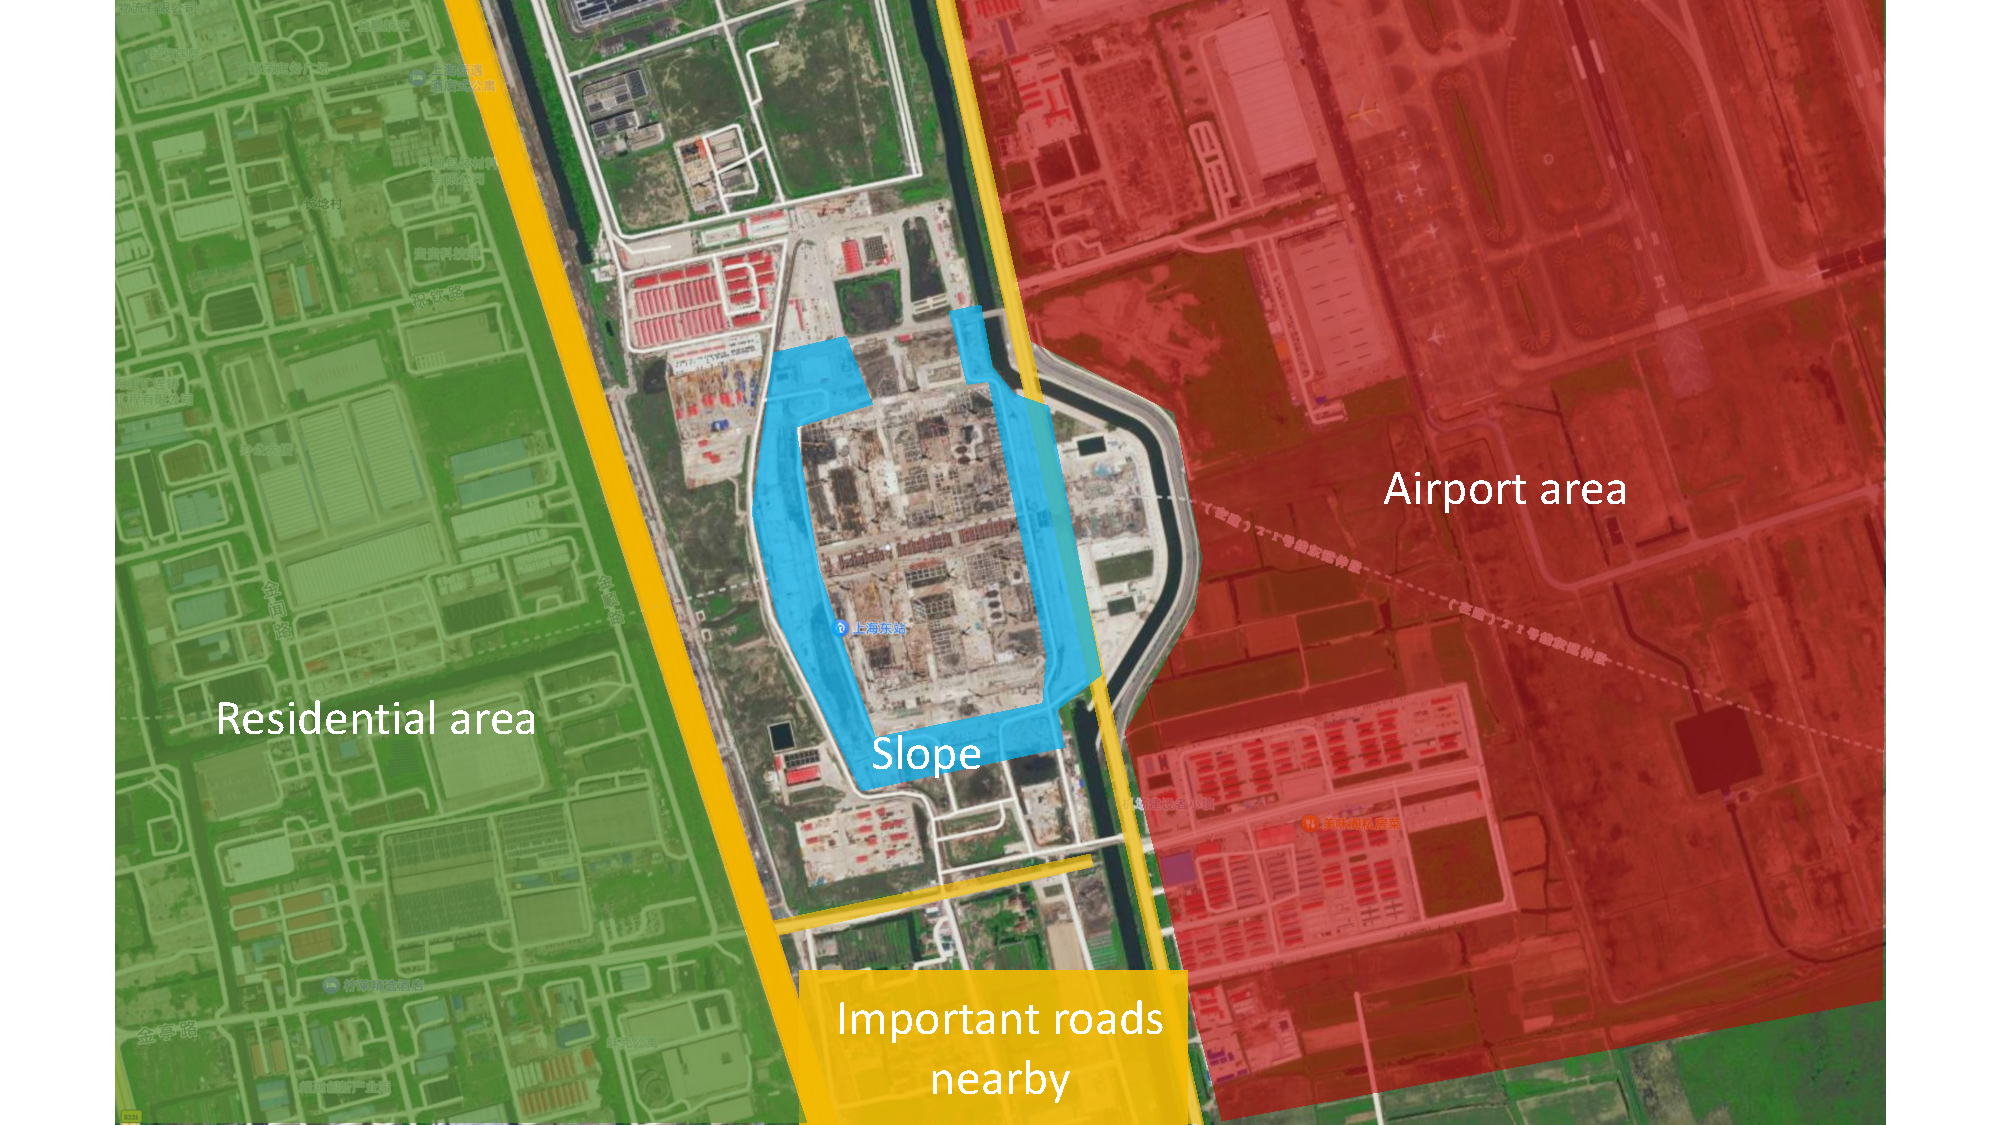
\includegraphics[width=0.9\textwidth]{imgs/Multi_chars.pdf}
    \caption{Complex environment around the excavation project of Shanghai East Railway Station}
    \label{fig:complexEnvironment}
\end{figure}

Over the past decade, a fused \textit{Space-Air-Ground} (\textbf{SAG}) paradigm—combining synthetic-aperture radar and optical satellites, unmanned-aerial-vehicle (UAV) photogrammetry/LiDAR, and in-situ sensor networks—has emerged as a credible solution to the trilemma. Bibliometric mining of 522 high-quality papers reveals a seven-fold expansion of "InSAR" and a five-fold expansion of "UAV" articles between 2006 and 2025, signalling rapid adoption of sky- and air-based technologies in geotechnical practice. Field evidence corroborates these trends: dual- or tri-modal SAG deployments routinely constrain wall-top displacement forecasts within $\pm2$ mm or $<10\%$ error while cutting life-cycle monitoring costs by an order of magnitude—for example, Persistent-Scatterer InSAR replaced \emph{thousands} of optical prisms during the post-excavation phase of London's Crossrail project, and at Shanghai East Railway Station a ground-only inclinometer array costed at USD 0.66 million was avoided through SAG substitution.

Despite these achievements, four critical gaps persist:
(i) sensor-physics limits under dense urban clutter,
(ii) heterogeneous data streams exceeding 5 GB d$^{-1}$ that outstrip manual analysis,
(iii) fragmented regulations that hinder cross-platform interoperability, and
(iv) long-term reliability issues over multi-year construction programmes.
Addressing these challenges demands a holistic perspective that integrates codes, sensing
principles, data-fusion analytics and digital-twin decision support.

This state-of-the-art review distils a fragmented knowledge landscape into an application-oriented
framework for large-scale deep excavations. We

\begin{enumerate}
  \item catalogue global and national codes that prescribe deformation indicators and precision
        requirements—e.g.\ ISO 18674-1, GB 50497-2019 and JGJ 120-2012—for SAG deployments;
  \item contrast the capabilities and limitations of the core sensing modalities (InSAR, UAV
        photogrammetry/LiDAR, GNSS and conventional geotechnical instruments) and identify their
        complementary niches;
  \item review eight mainstream data-fusion families—from Kalman filtering to deep learning—and
        map them to excavation monitoring scenarios;
  \item extract lessons from representative case studies across Asia and Europe, emphasising
        cost-benefit ratios and operational pitfalls; and
  \item outline research frontiers such as physics-informed deep fusion, edge-cloud analytics and
        autonomous "sensor-swarm" orchestration.
\end{enumerate}

The structure of this review is as follows:
Section 2 details the literature-search protocol and bibliometric results.
Section 3 surveys monitoring technologies and relevant standards;
Section 4 analyses multi-source data-fusion strategies;
Section 5 presents engineering case studies; and
Section 6 discusses persisting challenges and future directions.

\section{Literature-Search Protocol and Bibliometric Results}

This chapter documents the systematic approach adopted to identify, screen, and profile state-of-the-art research on Space-Air-Ground (SAG) monitoring for deep and large excavations (DLE). The workflow complies with the \textsc{PRISMA-ScR} checklist for scoping reviews \citep{PRISMA-ScR}. 
Considering that SAG integrated monitoring technologies are applicable far beyond excavations, the scope of the literature search was expanded to the broader field of geotechnical engineering. When defining search queries in the Web of Science (WoS) database, both the characteristic technologies of SAG monitoring and the common monitoring objectives were taken into account. The final query adopted was: 

\begin{quote}
\texttt{TS=("deep excavation" OR "foundation pit" OR Geotechnical) AND
TS=("InSAR" OR "satellite radar" OR UAV OR "drone photogrammetry" OR LiDAR) AND
TS=("monitoring" OR deformation OR safety)}
\end{quote}

Using the above query, a total of 687 records were retrieved from the Web of Science (WoS) Core Collection on 26 May 2025, as illustrated in \autoref{fig:retrieval}; these comprised 13 review papers and 36 doctoral or master's theses.  In order to pinpoint the most representative and application-oriented studies, a two-stage screening procedure was adopted.

\begin{enumerate}
    \item \textbf{Quality filter:} Journals were ranked according to the Chinese Academy of Sciences (CAS) quartile system; only Zone I-III outlets, plus all theses, were retained.
    \item \textbf{Relevance filter:} Papers had to report at least \emph{one or more concrete-engineering case studies} (e.g. a metro interchange, transport hub or deep basement) with quantitative monitoring results or field-validated modelling. Purely conceptual discussions or laboratory-only tests were excluded at this stage.
\end{enumerate}

After applying both filters, 522 publications remained in the core corpus. This dual criterion not only guarantees a baseline research quality but also ensures that the review captures studies delivering real-world insights—a key
requirement for engineering decision support. The geographic distribution of these publications is summarised in \autoref{fig:NationalStatistcs}.

\begin{figure}[htbp]
    \centering
    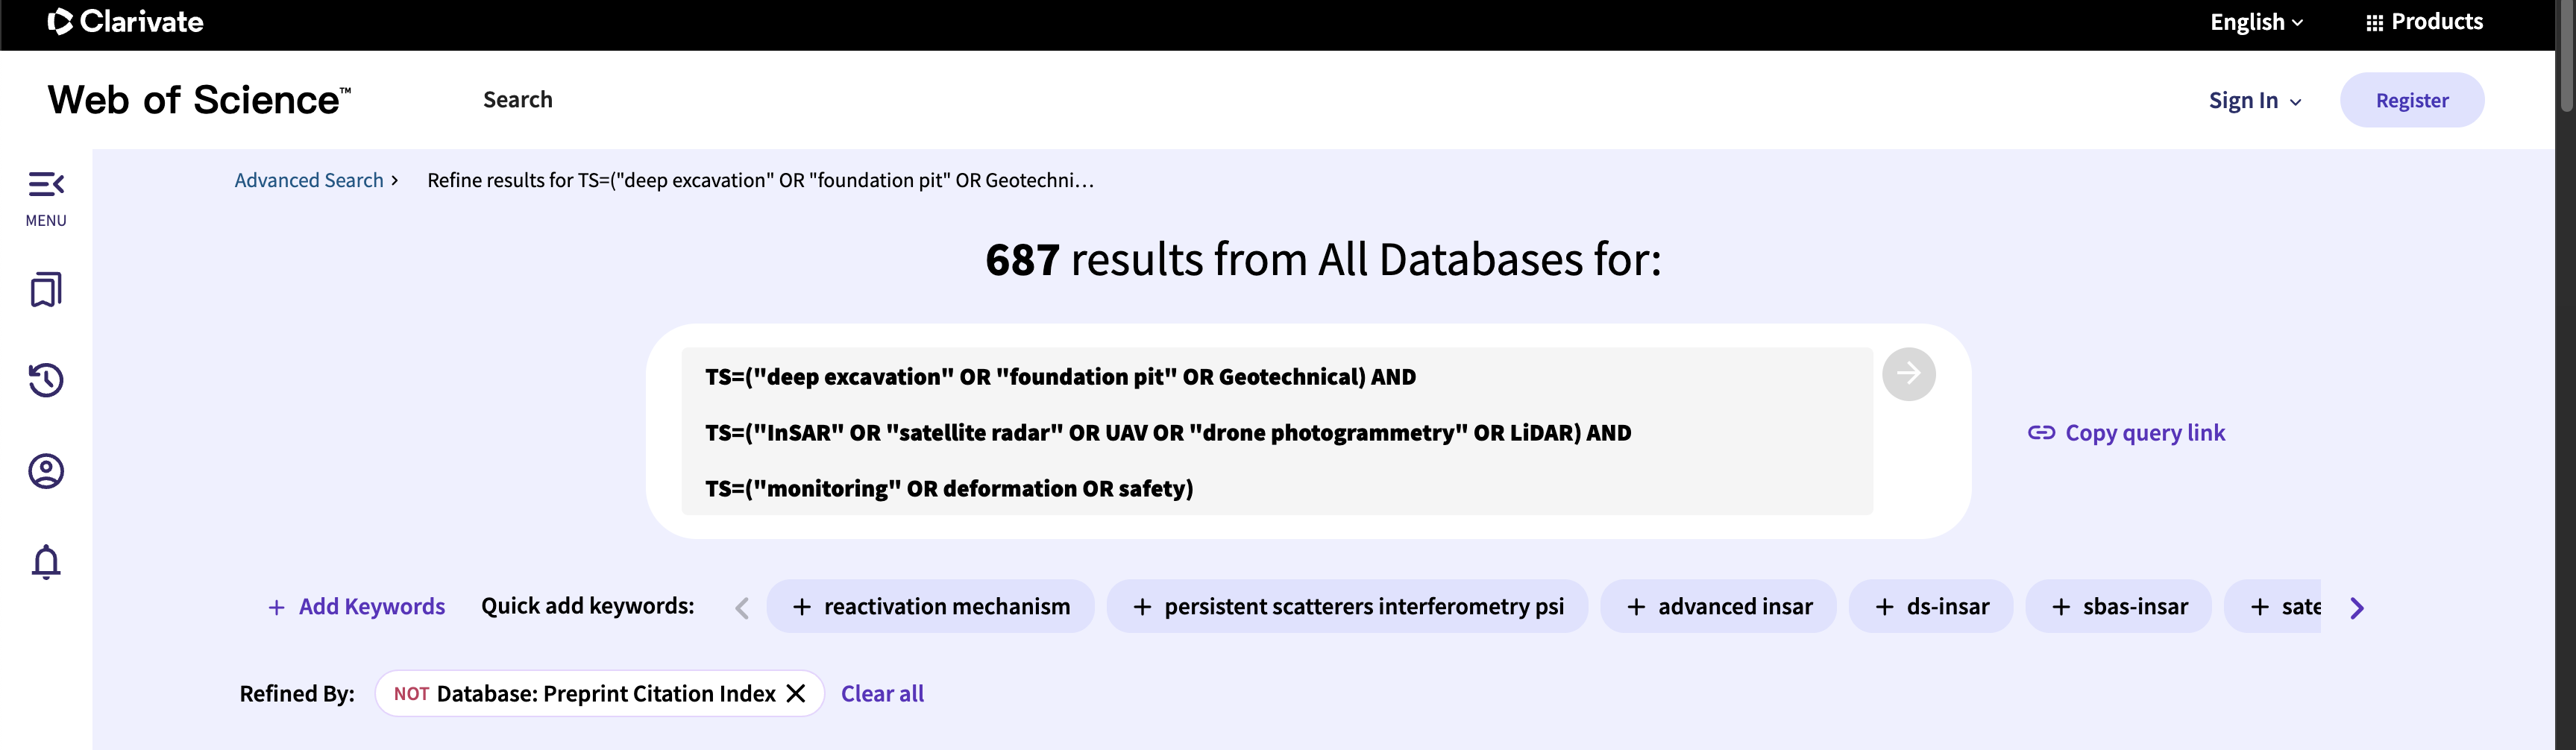
\includegraphics[width=\textwidth]{imgs/advanceSearch.png}
    \caption{Schematic diagram of retrieval results}
    \label{fig:retrieval}
\end{figure}

\begin{figure}[h]
    \centering
    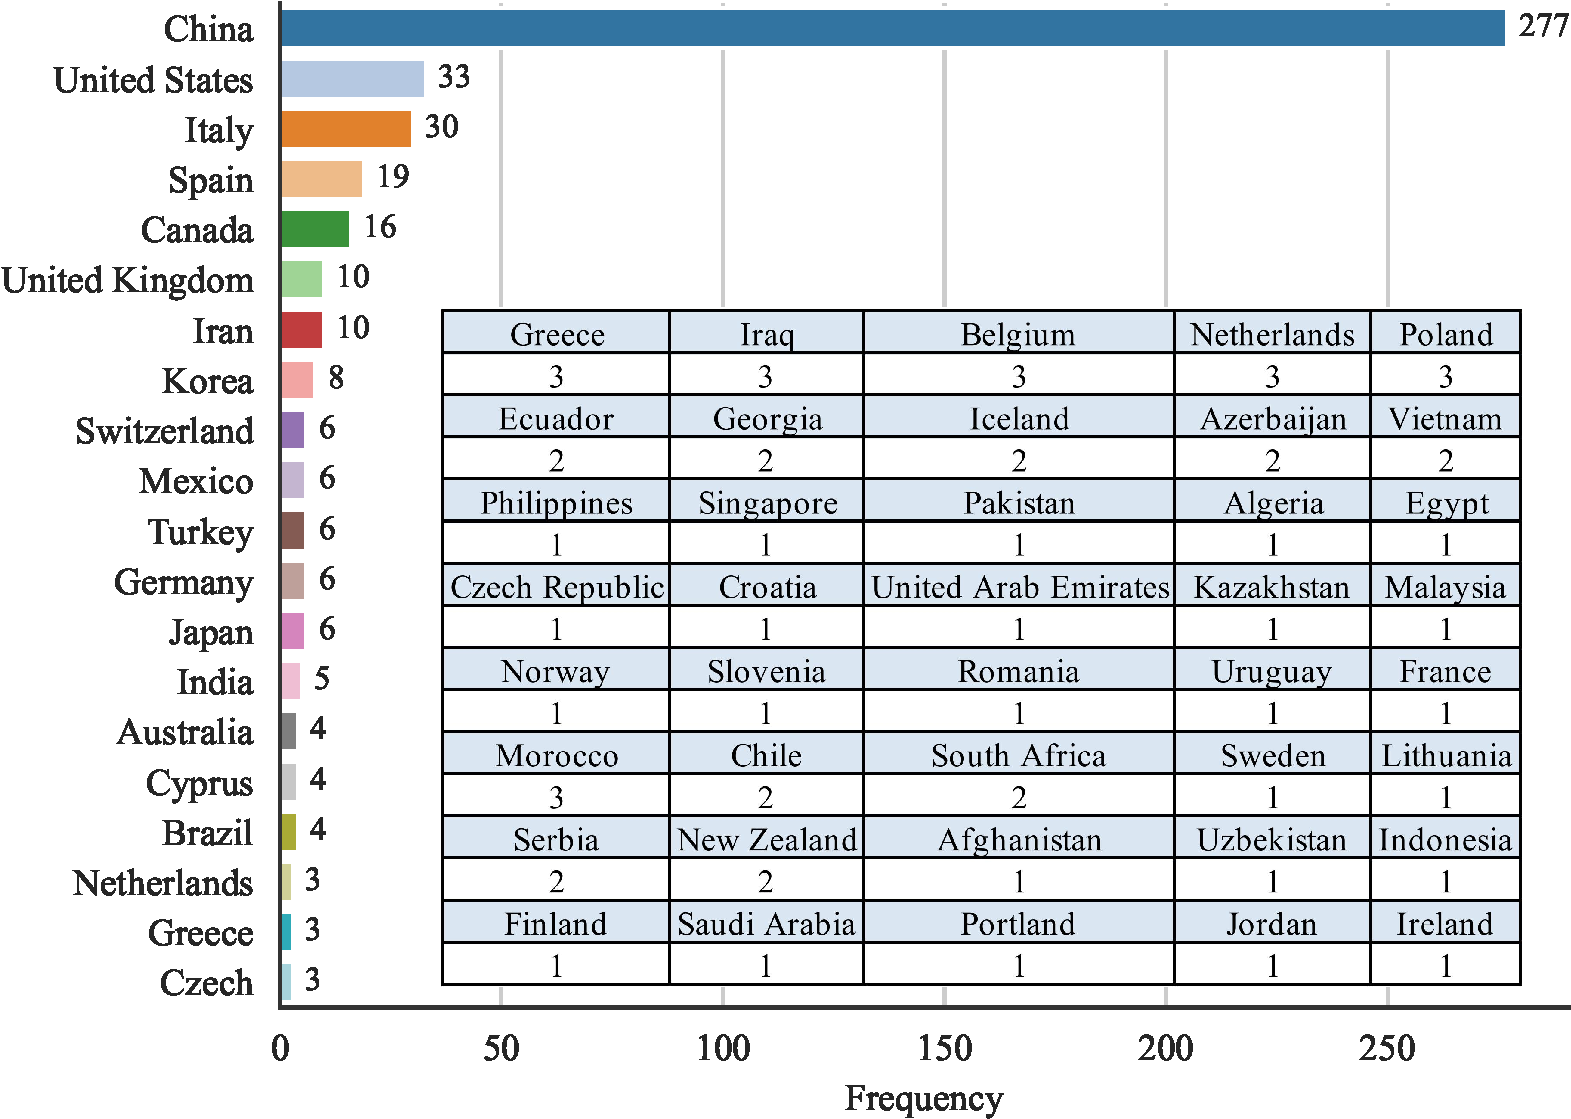
\includegraphics[width=\textwidth]{imgs/countries.pdf}
    \caption{National quantity statistics chart}
    \label{fig:NationalStatistcs}
\end{figure}

To reveal application trends, this papar annotated each paper with its engineering-project context and year of publication. Project contexts were categorised as: \emph{excavation} (deep-pit monitoring), \emph{bridge}, \emph{dam} (hydraulic infrastructure), \emph{flood}, \emph{mining}, \emph{slope}, \emph{tunnel}, \emph{roadbed}, \emph{urban} (urban infrastructure), and \emph{general} (general studies without a specific project). As depicted in \autoref{fig:YearProject}, the number of civil-engineering studies employing SAG monitoring has risen sharply year-on-year, indicating its progressive diffusion into structural-safety practice. The dominant project types are \emph{slope}, \emph{dam}, \emph{roadbed}, \emph{urban}, and \emph{mining}. While less common for small-scale projects, SAG shows significant potential in large excavations that often integrate \emph{slope}, \emph{roadbed}, and \emph{urban} elements.

\begin{figure}[htbp]
    \centering
    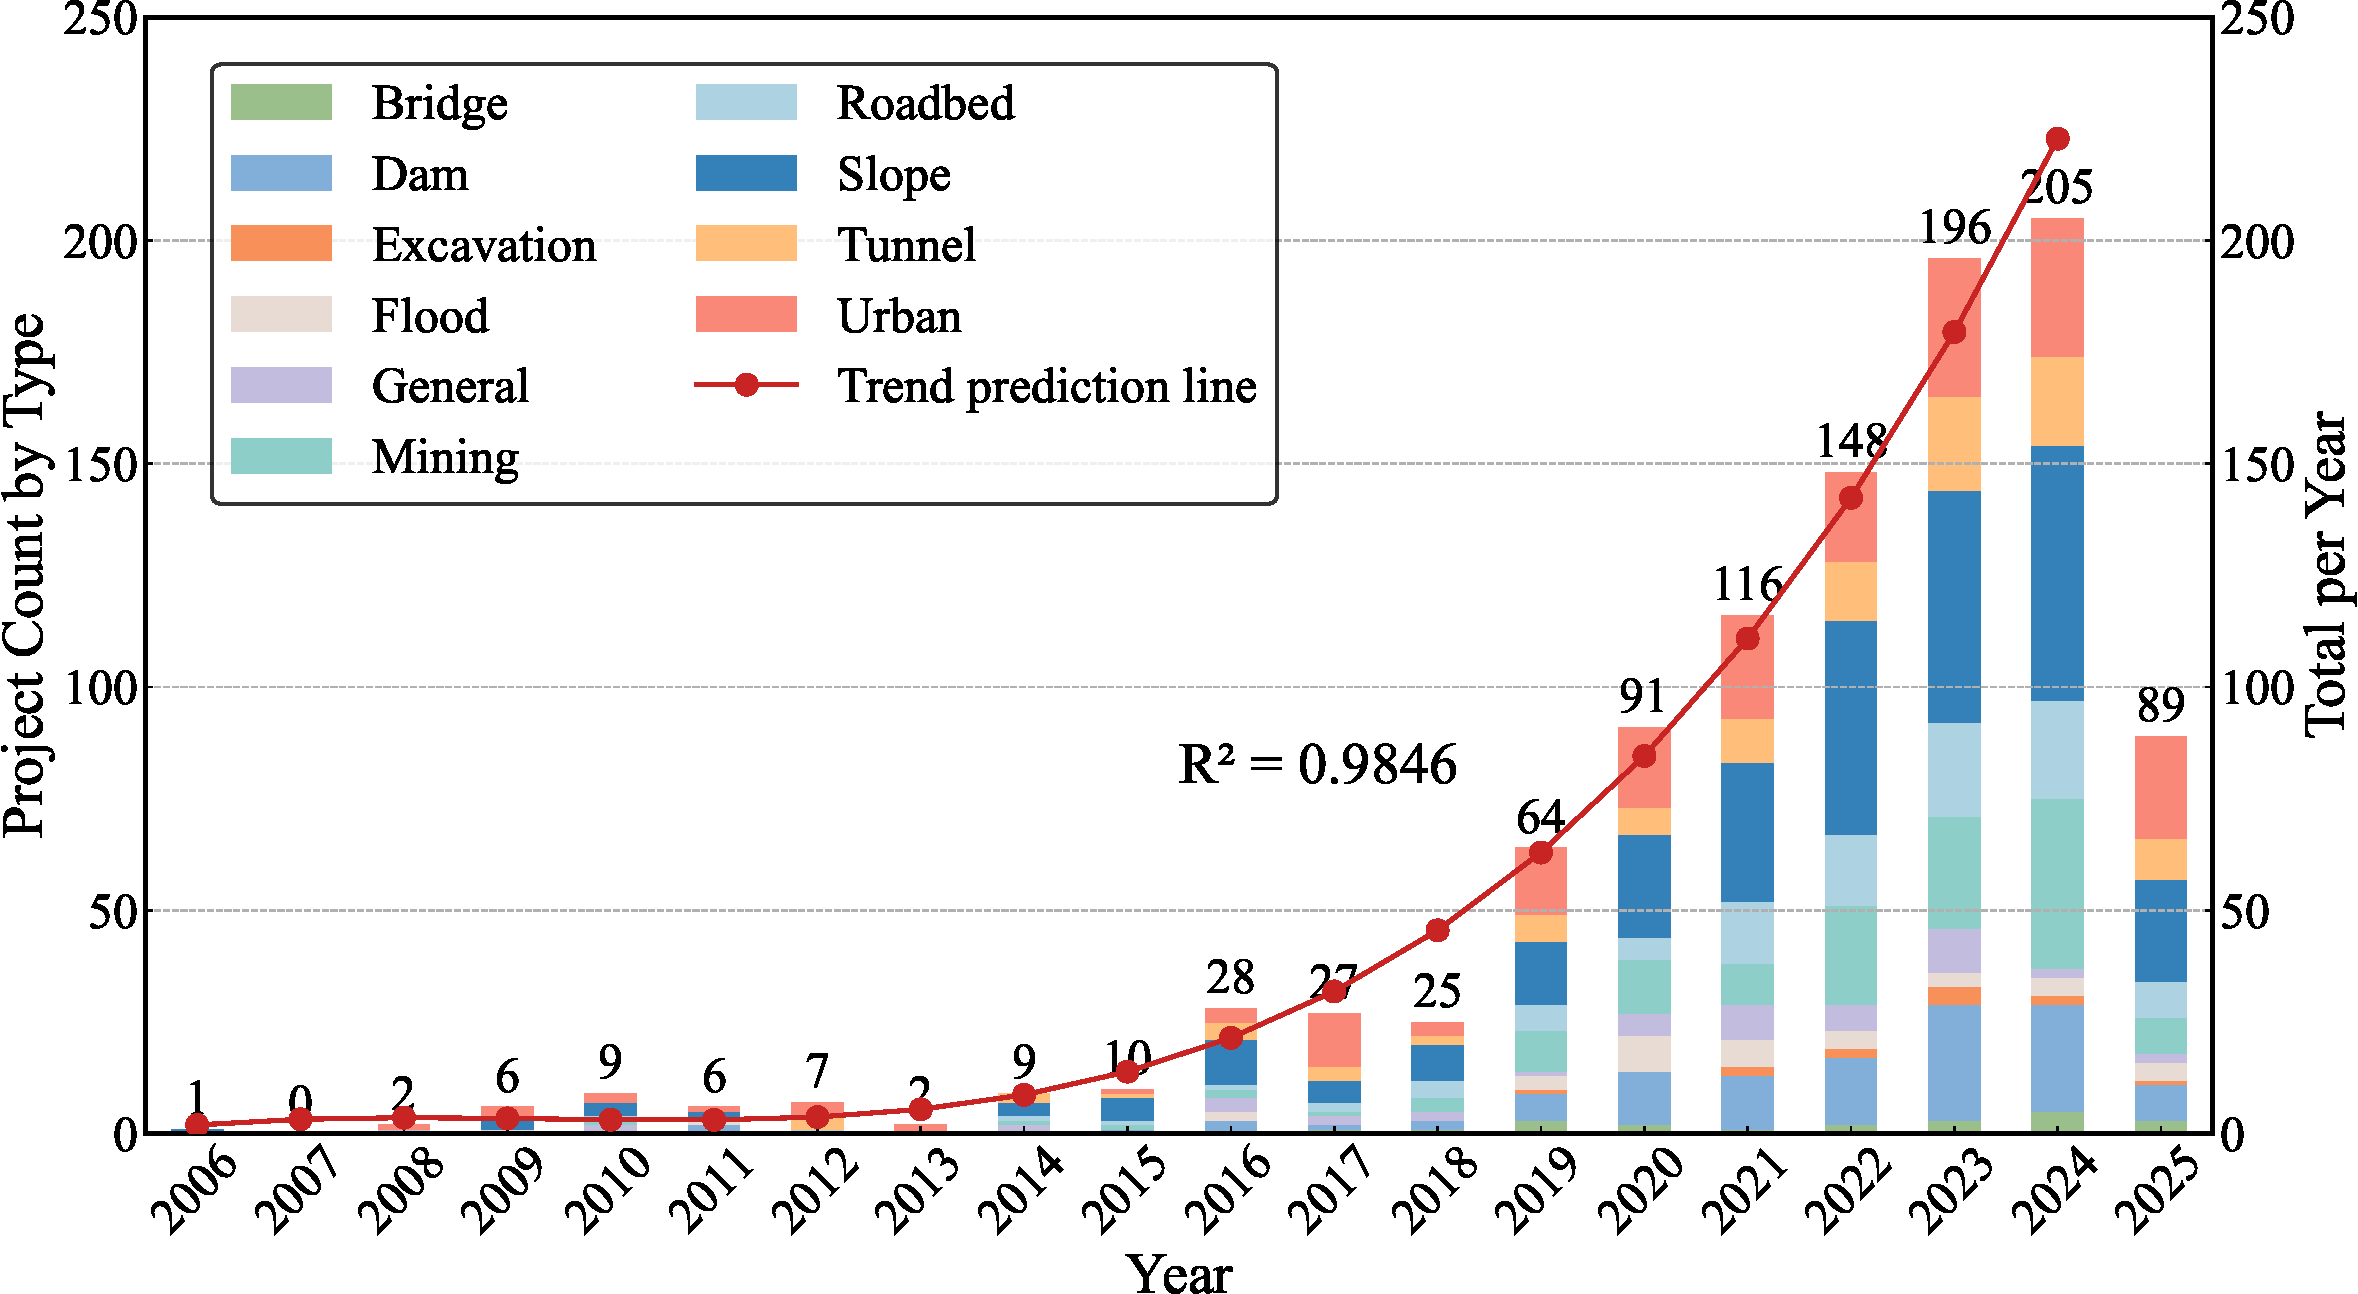
\includegraphics[width=\textwidth]{./imgs/Year_Types.pdf}
    \caption{Statistical chart of year and project types quantity with trend line}
    \label{fig:YearProject}
\end{figure}

To analyze the evolution of monitoring technologies, individual techniques were consolidated into broader categories: \emph{InSAR} (synthetic-aperture-radar deformation monitoring); \emph{GNSS (GPS)} (global navigation satellite systems); \emph{UAV} (optical remote-sensing from UAVs, terrestrial cameras, and satellites); \emph{LiDAR} (airborne and terrestrial laser scanning); and \emph{Ground} (proximity-sensing methods). As shown in \autoref{fig:YearTech}, the usage of \emph{LiDAR}, \emph{InSAR}, and \emph{UAV} has grown steadily, whereas \emph{Ground} and \emph{GNSS} applications are stable or slightly declining. This shift is likely driven by falling sensor costs and increasing automation. Within the SAG framework, \emph{InSAR} and \emph{UAV} have emerged as core monitoring solutions.

\begin{figure}[htbp]
    \centering
    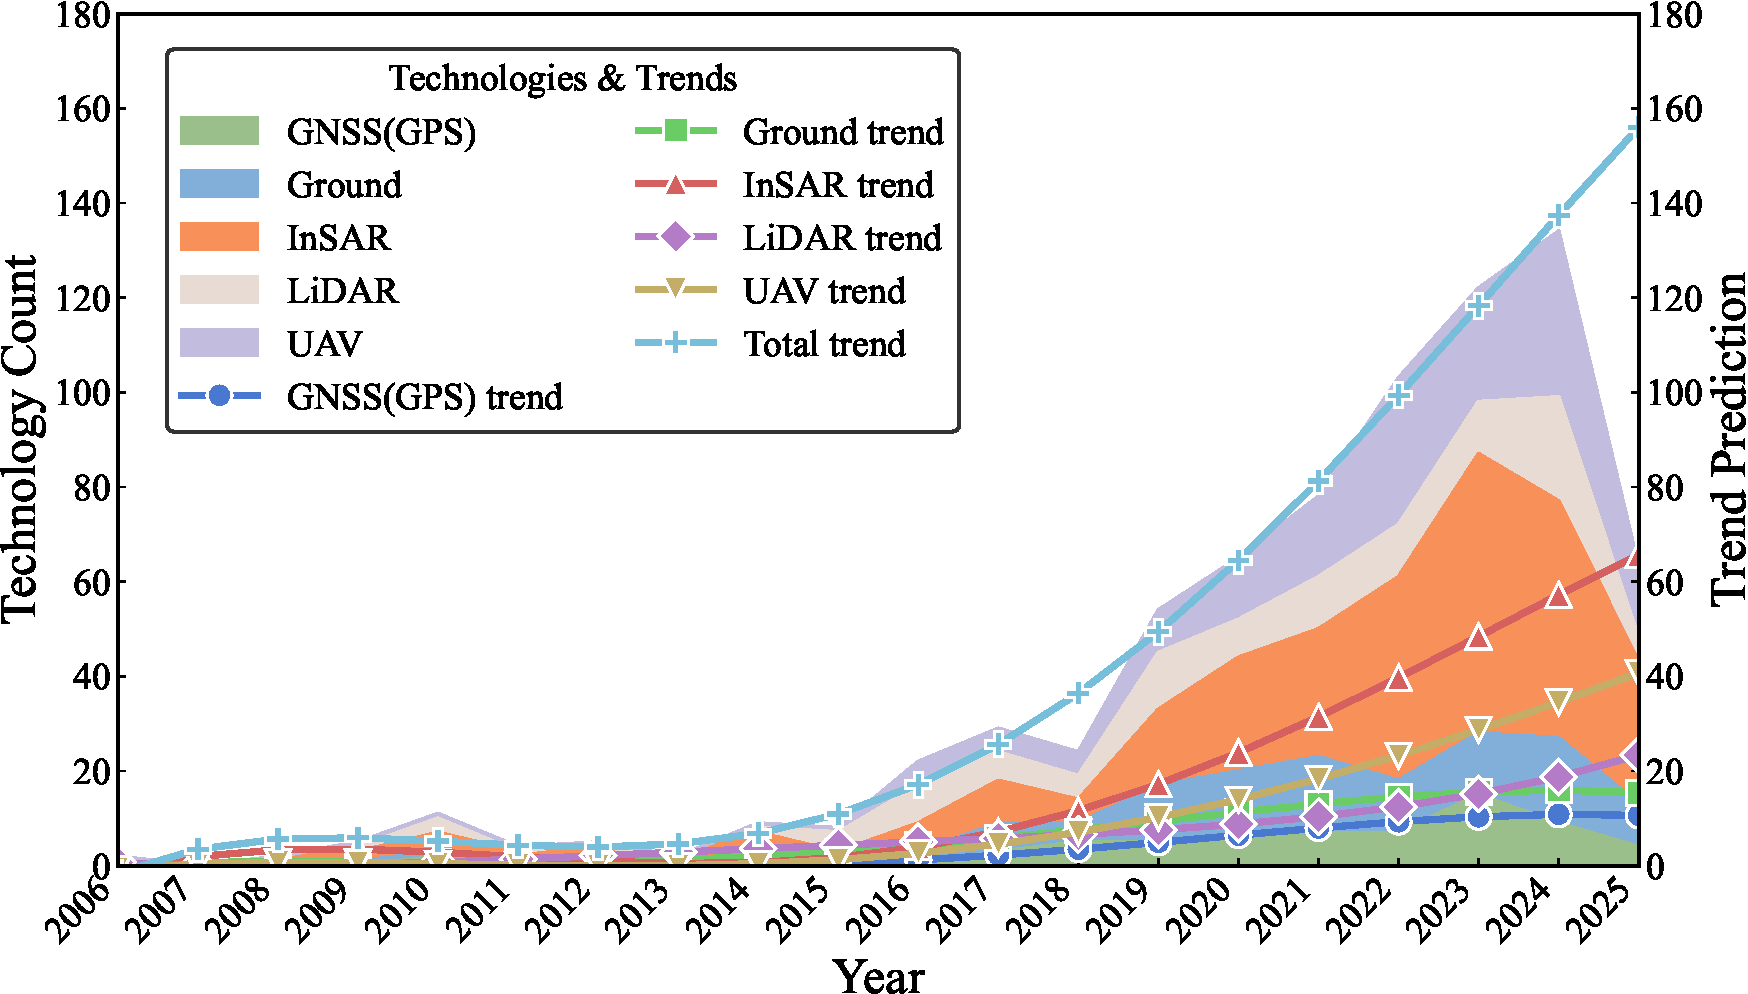
\includegraphics[width=\textwidth]{./imgs/Year_Tech.pdf}
    \caption{Statistical chart of year and technologies quantity with trend line}
    \label{fig:YearTech}
\end{figure}

To trace the evolution of research hotspots, a keyword co-occurrence analysis was conducted using a time-slicing approach (\citep{Lee01042010}). Three periods were analyzed: 2010-2014, 2015-2019, and 2020-2025. The resulting networks (\autoref{fig:CooccurrenceAnalysis}) and community analysis (\autoref{tab:Co_Nx}) confirm that both SAG technologies and their applications have diversified over time. Quantitative analysis (\autoref{tab:QuantitativeAnalTab}) further reveals that advanced techniques like \emph{InSAR} and \emph{UAV} have expanded from general surface-subsidence observation to applications in dam operation, tunnel construction, and smart-city management.


\begin{figure}
    \subfigure[2010-2014·Top 30 keywords·communities=5]{
        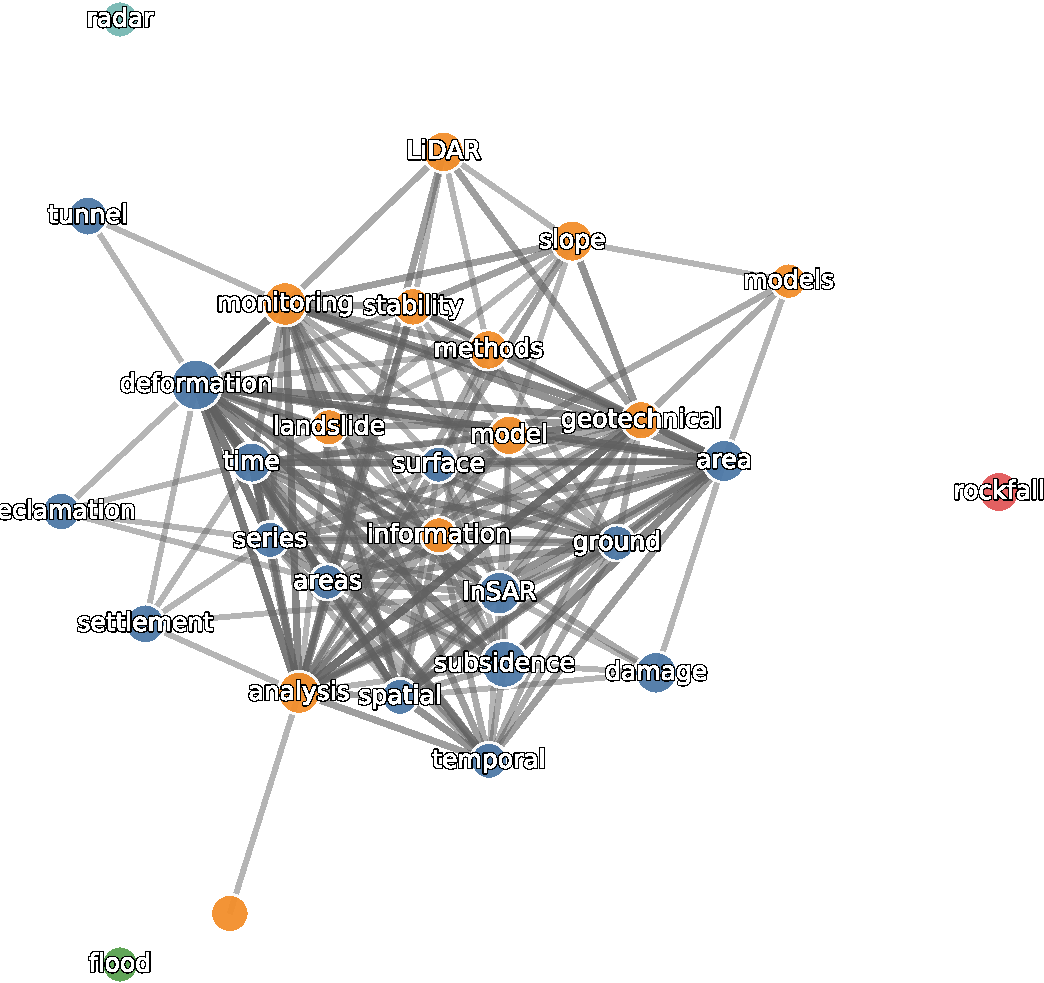
\includegraphics[width=0.5\textwidth]{imgs/keyword_network_2010-2014.pdf}
    }
    \hfill
    \subfigure[2015-2019·Top 30 keywords·communities-3]{
        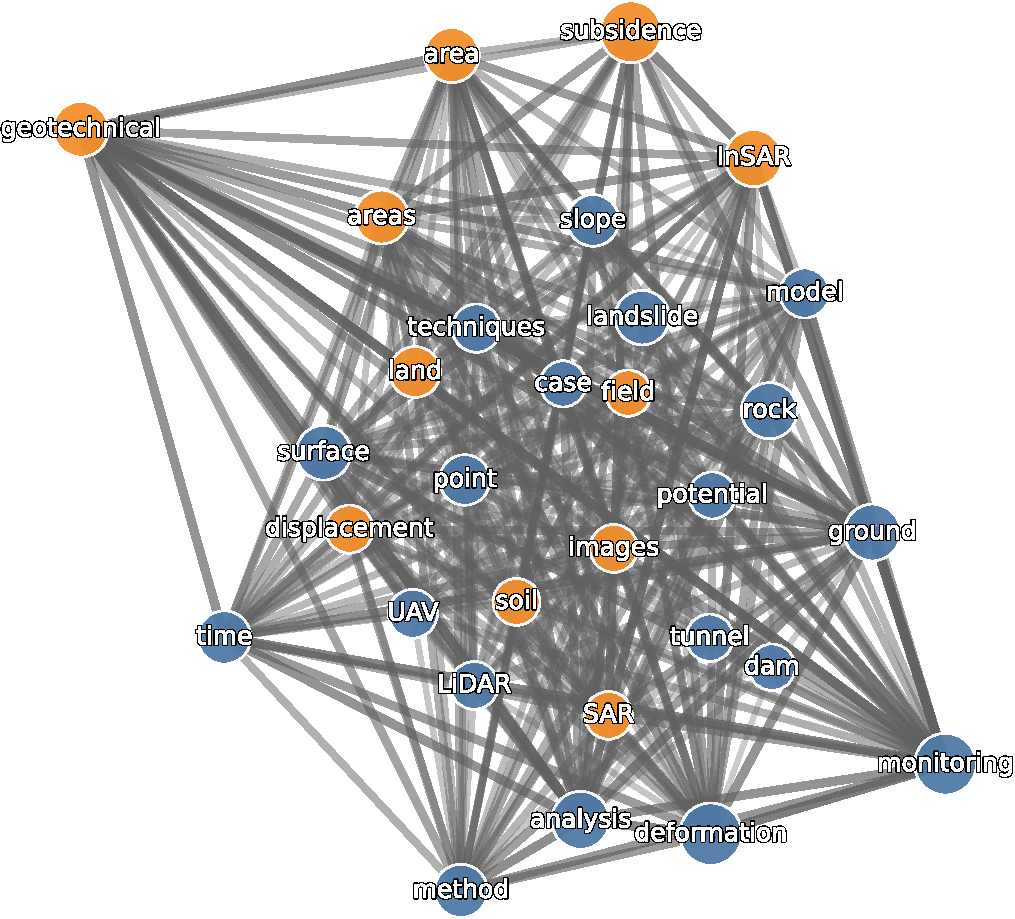
\includegraphics[width=0.5\textwidth]{imgs/keyword_network_2015-2019.pdf}
    }
    \hfill
    \subfigure[2020-2025 ·Top 30 keywords·communities-3]{
        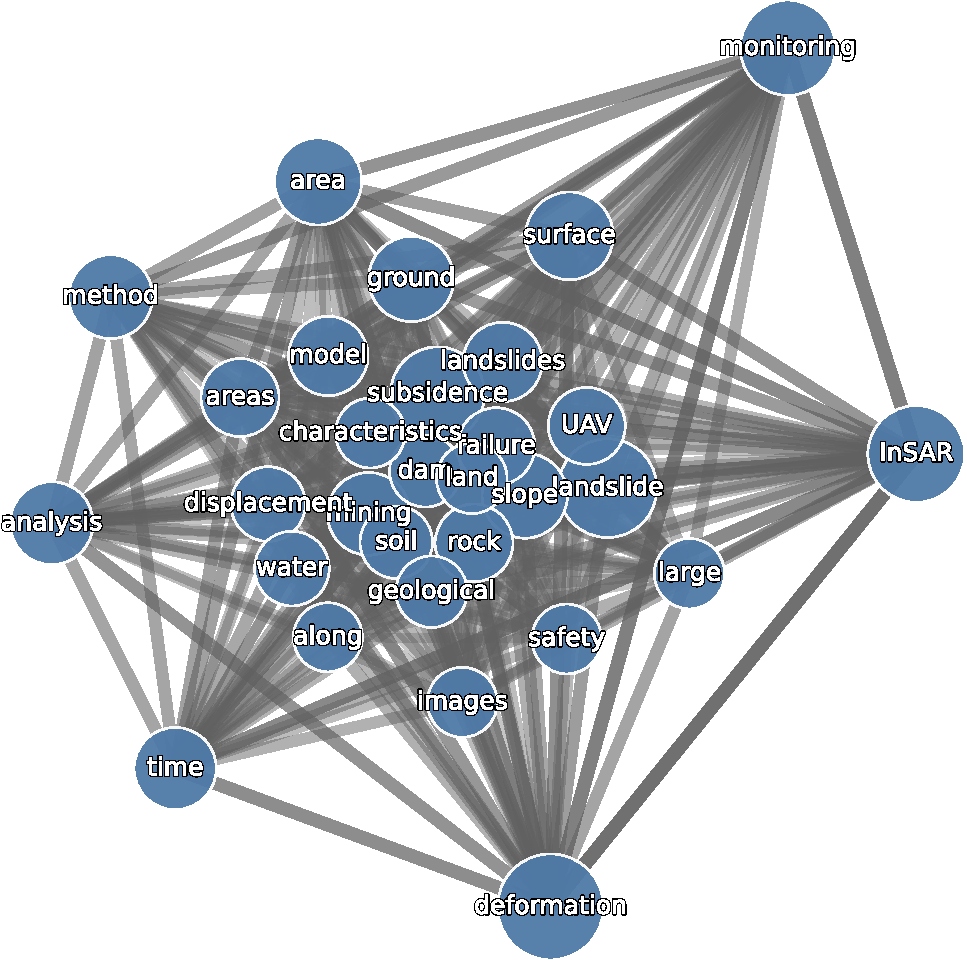
\includegraphics[width=0.5\textwidth]{imgs/keyword_network_2020-2025.pdf}
    }
    \caption{Co-occurrence analysis diagram of community identification keywords in different time periods}
    \label{fig:CooccurrenceAnalysis}
\end{figure}

\begin{table}[htbp]
    \centering
    \caption{Temporal evolution of the keyword co-occurrence network}
    \label{tab:Co_Nx}
    % 通过为前5列设置p{width}来精确控制其宽度
    % >{\centering\arraybackslash} 用于使p列内容居中
    \begin{tabularx}{\textwidth}{@{} p{4.5em} >{\centering\arraybackslash}p{5em} >{\centering\arraybackslash}p{3.5em} >{\centering\arraybackslash}p{3.5em} >{\centering\arraybackslash}p{6em} X @{}}
        \toprule
        \textbf{Period} & \textbf{Publications} & \textbf{Nodes} & \textbf{Edges} & \textbf{Communities} & \textbf{Key observations} \\
        \midrule
        2010--2014 & 22  & 25 & 166 & 3 & The early network is relatively sparse; topics such as \textit{LiDAR}, \textit{tunnel} and \textit{settlement} remain largely independent, exhibiting a multi-core structure. \\
        
        2015--2019 & 92  & 25 & 287 & 1 & With the surge in publications, connections among core high-frequency terms become markedly denser, community boundaries blur, and a single dense mega-cluster forms; the themes "monitoring-data-deformation" are tightly coupled and SAG spreads rapidly in multiple scenarios. \\
        
        2020--2025 & 403 & 25 & 300 & 1 & Node degree and size continue to rise, and the network approaches a "highly integrated" configuration. New terms such as \textit{UAV}, \textit{InSAR}, and \textit{mining} enter the Top-25 list but are rapidly absorbed into the main community, indicating strong cross-fertilization and convergence of the thriving research topics. \\
        \bottomrule
    \end{tabularx}
\end{table}

\begin{table}[htbp]
  \centering
  \caption{Quantitative analysis table of keyword co-occurrence}
  % 使用 tabularx 并设置总宽度为页面宽度
  % l: 第一列左对齐
  % *{5}{...}: 将括号内的列格式重复5次
  % >{\centering\arraybackslash}X: 创建一个内容居中的、可自动伸缩的X列
  \begin{tabularx}{1.05\textwidth}{@{} l *{5}{>{\centering\arraybackslash}X} @{}}
    \toprule
    \textbf{Keyword} & \textbf{2010-2014} & \textbf{2015-2019} & \textbf{Growth\_2015-2019} & \textbf{2020-2025} & \textbf{Growth\_2020-2025} \\
    \midrule
    \textbf{InSAR} & 23      & 70      & 204.3\% & 582     & 731.4\% \\
    \textbf{slope} & 22      & 48      & 118.2\% & 374     & 679.2\% \\
    \textbf{UAV} & 0       & 38      & -       & 232     & 510.5\% \\
    \textbf{dam} & 10      & 36      & 260.0\% & 211     & 486.1\% \\
    \textbf{subsidence} & 35      & 101     & 188.6\% & 562     & 456.4\% \\
    \textbf{displacement} & 7       & 39      & 457.1\% & 212     & 443.6\% \\
    \textbf{ground} & 13      & 74      & 469.2\% & 374     & 405.4\% \\
    \textbf{tunnel} & 18      & 35      & 94.4\% & 166     & 374.3\% \\
    \textbf{infrastructure} & 4       & 27      & 575.0\% & 82      & 203.7\% \\
    \textbf{urban} & 5       & 33      & 560.0\% & 70      & 112.1\% \\
    \bottomrule
  \end{tabularx}
  \label{tab:QuantitativeAnalTab}
\end{table}

To provide practical guidance for using SAG technology in excavation monitoring, the following sections will:

\begin{enumerate}
    \item Review relevant standards and codes for monitoring parameters and precision control.
    \item Detail SAG monitoring methodologies identified from the literature.
    \item Analyze the salient characteristics of diverse monitoring technologies.
    \item Summarize established approaches for integrating heterogeneous, multi-source data.
\end{enumerate}

\section{Technology Background and Methodological Framework}

This chapter frames Space-Air-Ground (SAG) monitoring for deep and large excavations (DLEs) from four perspectives—\emph{regulatory context}, \emph{space-based sensing}, \emph{air-based sensing}, and \emph{ground-based instrumentation}. A sensor-selection matrix concludes the chapter, matching project scale to an optimal device mix.

\subsection{Regulatory Landscape of SAG-Enabled Excavation Monitoring}

Modern megacity excavations exceed 30\,m in depth and often sit within sub-metre clearance of critical utilities,turning deformation control from an \emph{"as-built check"} into a \emph{"design-integral function"}. Consequently, regulations worldwide are shifting from manual instrumentation plans toward automated, multi-sensor schemes that now explicitly reference satellite, UAV and IoT data streams.

ISO 18674-1:2015 standardises terminology and requires monitoring plans to include documented trigger-action levels, while the subsequent parts of the ISO 18674 series (e.g., Parts 3-5) set instrument-specific performance criteria such as measurement range, accuracy and repeatability \citep{ISO18674-1:2015, ISO18674-2:2016, ISO18674-3:2017, ISO18674-4:2020, ISO18674-5:2019, ISO18674-6:2025, ISO18674-7:2024, ISO18674-8:2023}. Eurocode 7 (EN 1997-1:2024) defines the Observational Method, stipulating (i) predefined prediction limits, (ii) rapid feedback of monitoring data and (iii) pre-approved mitigation measures \citep{EN1997-1:2024}. Neither standard prescribes how orbital or aerial observations should be integrated with ground-based sensors, leaving this fusion to national or project-level guidelines.

\begin{itemize}

    \item \textbf{China.} GB 50497-2019 and JGJ 120-2012 list InSAR and UAV photogrammetry as approved settlement tools; Shanghai's 2023 local addendum fixes a 5 m sensor grid for pits $>30$ m \citep{GB50497:2019,ShanghaiAddendum2023}.

    \item \textbf{United Kingdom.} CIRIA C760 pairs the OM with a colour-coded trigger ladder and explicitly recommends automated total stations (AMTS) and UAV mapping \citep{CIRIA760}.

    \item \textbf{Germany.} DIN 1054 aligns with Eurocode 7 but adds a clause on digital twins for excavation control \citep{DIN1054:2021-04}.
    
    \item \textbf{Australia.}  The National Construction Code (NCC 2022) defers to Australian Standards AS 1726-2017 (\emph{Geotechnical Site Investigations}) and AS 4678-2019 (\emph{Earth-Retaining Structures}), both of which require baseline and staged monitoring; recent state-level specs—e.g. Queensland \emph{Geotechnical Design Standard - Minimum Requirements} (2024) and South Australia DIT “ST-PI-C4 Diaphragm Walls” (2024)— mandate inclinometer arrays, trigger-action levels and web-based data push for deep basements \citep{AS1726,TMR2024,DIT2024}.

    \item \textbf{Singapore.} BCA "Rigorous Approach" (2022) enforces 24/7 data streaming and site video for works $\ge$ 5 million, advocating UAV-BIM integration \citep{BCA_Rigorous_Approach_2022}.
  
    \item \textbf{USA/Canada.} FHA (1998) and CFEM (2019) still focus on conventional ground arrays; SAG adoption remains project-driven \citep{FHWA:GEC:Series,CFEM:2023}.

\end{itemize}

\begin{table}[htbp]
\centering\small
\caption{Key excavation-monitoring codes and their provisions for automated
         and SAG sensing (\checkmark = explicit, $\triangle$ = optional,
         — = absent).}
\label{tab:codes_compare}
\begin{tabular}{@{}lllll@{}}
\toprule
\textbf{Code} & \textbf{Year} & \textbf{OM$^{\dagger}$ / TAL$^{\ddagger}$} &
\textbf{InSAR / UAV} & \textbf{Data push} \\
\midrule
ISO 18674-1   & 2015 & $\triangle$ & —            & — \\
EN 1997-4     & 2007 & \checkmark & —            & — \\
GB 50497      & 2019 & \checkmark & \checkmark   & $\triangle$ \\
CIRIA C760    & 2019 & \checkmark & $\triangle$  & $\triangle$ \\
BCA (SG)      & 2022 & \checkmark & \checkmark   & \checkmark \\
DIN 1054      & 2021 & \checkmark & $\triangle$  & — \\
AS 1726 / AS 4678 & 2017 / 2019 & \checkmark & $\triangle$ & $\triangle$ \\
TMR (QLD) GDS-MR & 2024 & \checkmark & $\triangle$ & \checkmark \\
CFEM          & 2019 & $\triangle$ & —            & — \\
\bottomrule
\end{tabular}
\begin{tablenotes}\footnotesize
\item $^{\dagger}$OM = Observational Method;
      $^{\ddagger}$TAL = Trigger-Action Level.
\end{tablenotes}
\end{table}
% \footnotetext{OM = Observational Method; TAL = Trigger-Action Level.}

Based on the above research and analysis, the following points are summarized: Deep excavations impose three non-negotiable requirements: \emph{(i) latency} - sampling intervals from seconds to a few minutes to capture rapid failure modes; \emph{(ii) density} — 5-10 m grid spacing near diaphragm walls to detect localised deformation; and \emph{(iii) robustness} — sensors must withstand harsh construction activities such as blasting, jet-grouting, and TBM-induced vibration \citep{CIRIA760,ShanghaiAddendum2023}.  
SAG (Space-Air-Ground) frameworks address requirements (i) and (ii) by complementing sparse high-precision ground points with wide-area orbital and aerial observations. In addition, modality redundancy enhances overall system resilience by enabling cross-validation and mitigating single-sensor failure risks.
Global codes converge on risk-based, data-driven control, yet diverge in how explicitly they recognise satellite and UAV inputs. Current committee drafts (ISO /CD 18674-9 and the second-generation Eurocode 7 suite) acknowledge satellite and other remote-sensing methods, but they have not yet issued formal multi-sensor fusion procedures; national or project-specific guidance will still be required until such rules emerge.

\subsection{Principles and Characteristics of SAG Monitoring Technologies}\label{subsec:tech_principles}

This subsection dissects the physical principles and engineering attributes of the three sensing pillars that form a
\emph{SAG} monitoring stack (Fig. \ref{fig:sag_schematic}). A concise comparison matrix follows in Table~\ref{tab:sag_matrix}.

% \begin{figure}[htbp]
%   \centering
%   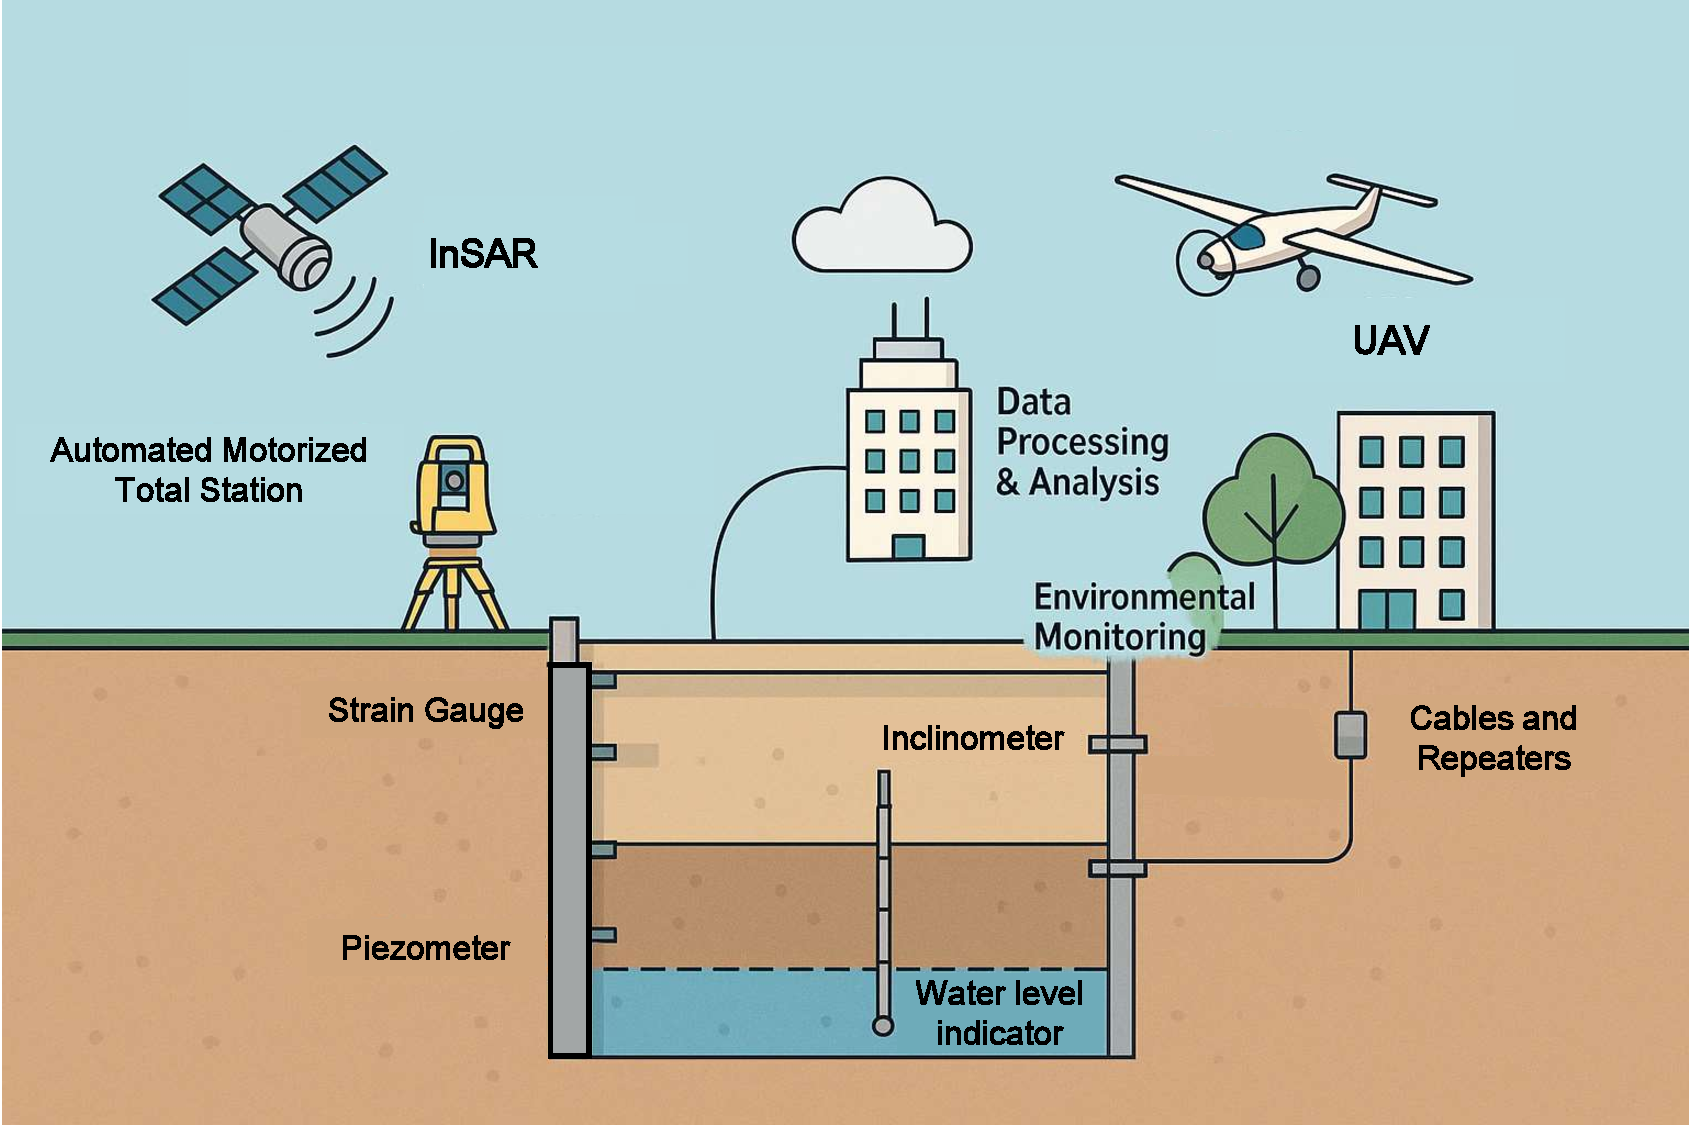
\includegraphics[width=\linewidth]{imgs/SAG_schematic.pdf}
%   \caption{Conceptual SAG monitoring stack for deep excavations
%            (LOS = line-of-sight, DEM = digital elevation model).}
%   \label{fig:sag_schematic}
% \end{figure}

\subsubsection{Space-borne InSAR}

Space-borne Interferometric Synthetic Aperture Radar (InSAR) is a powerful remote sensing technique for measuring ground surface deformation over large areas. Its physical principle is rooted in analyzing the phase of radar signals. The measured phase, $\varphi$, from a single SAR acquisition is a composite of the two-way slant range $\rho$, atmospheric delay $\varphi_{\text{atm}}$, and noise $\varphi_{\text{noise}}$, expressed as $\varphi = \tfrac{4\pi}{\lambda}\rho + \varphi_{\text{atm}} + \varphi_{\text{noise}}$, where $\lambda$ is the radar wavelength. By differencing the phase signals $\Delta\varphi$ from two or more repeat-pass satellite acquisitions (Fig.~\ref{fig:insar_principle}), the component related to topography can be removed, isolating the displacement along the satellite's line-of-sight (LOS). This displacement, $d_{\mathrm{LOS}}$, is calculated modulo $2\pi$ using:

\begin{align}
  d_{\mathrm{LOS}} = \frac{\lambda}{4\pi},\Delta\varphi
  \quad (\text{mod } 2\pi).
  \label{eq:insar}
\end{align}

To overcome phase ambiguity and atmospheric errors, multi-temporal InSAR techniques, such as Persistent Scatterer Interferometry (PSI) and Small Baseline Subset (SBAS), process a time-series of $\ge 20$ acquisitions. This allows for the robust retrieval of deformation histories with a precision of 1-3 mm at spatial resolutions typically ranging from 20-100 m \citep{Ferretti2014}.

From an engineering perspective, InSAR is characterized by its expansive coverage, with a single scene mapping tens to hundreds of square kilometers. Its revisit time (latency) varies from as short as half a day for high-resolution X-band spotlight imagery to a standard 12 days for sensors like Sentinel-1. However, its primary limitations include signal decorrelation in non-urban or vegetated areas, artifacts induced by atmospheric turbulence, and geometric distortions such as layover and shadow in steep terrain.

% \begin{figure}[htbp]
%  \centering
%  \includegraphics[width=0.9\linewidth]{imgs/InSAR_principle.pdf}
%  \caption{Simplified geometry of differential InSAR, illustrating the measurement of displacement between two satellite passes.}
%  \label{fig:insar_principle}
% \end{figure}

\subsubsection{Air-borne Photogrammetry and LiDAR}

The air-borne tier, predominantly utilizing Unmanned Aerial Vehicles (UAVs), offers high-resolution, on-demand mapping capabilities through two principal methods: photogrammetry and LiDAR.

UAV photogrammetry relies on the principles of stereopsis and triangulation. It involves processing a collection of overlapping nadir (top-down) and oblique images using Structure-from-Motion (SfM) and Multi-view Stereo (MVS) algorithms. These algorithms reconstruct the 3D geometry by back-projecting corresponding image points ((u,v)) through estimated camera projection matrices $\mathbf{P}i$ to solve for the 3D world coordinates $\mathbf{X} \in \mathbb{R}^3$. The process is formulated as a large-scale bundle adjustment optimization problem:

\begin{align}
    \min{\mathbf{X},,{\mathbf{P}i}}
    \sum{i=1}^{N} \lVert \mathbf{p}_i - \mathbf{P}_i\mathbf{X} \rVert^2.
\end{align}

When georeferenced with accurately surveyed ground-control points (GCPs) using RTK-GNSS, it is routine to achieve an absolute accuracy of 5-10 mm for a ground sampling distance (GSD) of 1 cm \citep{nwaogu2023application}.

UAV LiDAR (Light Detection and Ranging) operates on the time-of-flight principle. It emits laser pulses at a high pulse repetition frequency ($f_{\text{PRF}}$, typically around 640 kHz) and measures the round-trip time $\Delta t$ for each pulse to return to the sensor. The distance is then calculated as $R = \tfrac{c,\Delta t}{2}$, where $c$ is the speed of light. The raw point cloud is georeferenced in real-time using an onboard high-grade Inertial Navigation System (INS) and Inertial Measurement Unit (IMU). Subsequent post-processing, including strip-matching and bore-sight calibration, typically yields a vertical root-mean-square error (RMSE) of 8-15 mm for flight blocks covering 10-20 hectares.

The key attribute of UAV-based methods is their flexibility, enabling data acquisition with revisit times measurable in hours. They deliver exceptionally high resolution, with point cloud densities often exceeding 1000 points per square meter (pts $m^{-2}$). Their main limitations are susceptibility to adverse weather and high wind conditions, a critical dependency on the stability of GCPs for photogrammetry, and the potential for IMU drift and data noise in LiDAR.

\subsubsection{Ground-based Instrumentation}

The terrestrial tier of the SAG framework consists of in-situ instrumentation that provides high-frequency, high-precision measurements at discrete locations. Key technologies include:

Automated Motorized Total Stations (AMTS) operate based on Electronic Distance Measurement (EDM), which determines distance by analyzing the phase shift of a carrier wave. The distance $D$ is precisely calculated as $D = \frac{\lambda}{2}\left ( N + \frac{\Delta\phi}{2\pi} \right )$, where $N$ is the integer number of wavelengths and $\Delta\phi$ is the phase difference. Equipped with automatic target recognition and scheduling, AMTS systems can monitor a network of prisms with 2-3 mm precision at measurement intervals ranging from 1 to 15 minutes \citep{Dunnicliff2018}.

In-place inclinometers, typically using MEMS (Micro-Electro-Mechanical Systems) technology, are installed in boreholes to measure subsurface lateral displacements. The tilt angle $\theta$ at a specific depth is derived from the MEMS accelerometer output $\mathbf{a}$ via the relation $\theta = \arctan \big(\tfrac{a_y}{a_z}\big)$. By integrating these tilt measurements along the axis of the borehole, the cumulative deflection profile of a structure, such as a retaining wall, can be determined: $u(z) = \int_0^z \theta(s),ds$. This method can achieve a precision of 0.5-1 mm.

Global Navigation Satellite System (GNSS) receivers, utilizing Real-Time Kinematic (RTK) or Precise Point Positioning (PPP) techniques, provide continuous 3D coordinate monitoring. By differencing carrier-phase measurements between a rover and a reference station (or a network), ionospheric and other systematic errors are effectively mitigated. Modern dual-constellation (e.g., BDS-GPS) networks can routinely deliver 5-15 mm vertical accuracy at a sampling rate of 1 Hz, even within challenging urban canyons \citep{Li2023}.

In synthesis, the three tiers of the SAG monitoring paradigm offer powerfully complementary observational capabilities. Space-borne InSAR provides the synoptic, wide-area view, establishing regional settlement baselines and long-term trends. Air-borne photogrammetry and LiDAR bridge the gap by delivering high-resolution, meso-scale 3D models on an on-demand basis. Finally, ground-based sensors ensure project safety and structural integrity by providing high-precision, high-frequency local measurements and alerts. It is this synergy of complementary spatial and temporal scales that validates the adoption of a tri-modal SAG framework. The principles and characteristics detailed herein lay the physical groundwork for the multi-sensor data fusion algorithms that will be presented in Section \ref{sec.fusion}, which are shown in \autoref{tab:sag_principle}.

% 表二:Principle-feature matrix(保留精度/覆盖率/延迟等)
\begin{landscape}
\begin{table}[htbp]
\centering\small
\caption{Principle-feature matrix of SAG sensors (typical performance parameters).}
\label{tab:sag_principle}
\begin{tabular}{@{}p{2.8cm}p{3cm}p{2.8cm}p{2.5cm}p{2.5cm}p{8cm}@{}}
\toprule 
\textbf{Modality} & \textbf{Core principle} & \textbf{Coverage} & \textbf{Precision} & \textbf{Latency} & \textbf{Performance highlights / limitations} \\
\midrule
InSAR (C/X-band) & Phase differencing, \autoref{eq:insar} & 10-400 km$^2$ & 1-5 mm LOS & 0.5-12 d & Cost-effective for large areas, ideal for cumulative trends; sensitive to decorrelation and layover. \\
UAV Photogrammetry & SfM triangulation & 0.5-5 ha & 5-15 mm & 3-6 h & Captures rich textures and surface detail; weather-sensitive, requires stable GCPs. \\
UAV LiDAR & Time-of-flight + INS alignment & 0.2-3 ha & 8-15 mm (z) & 2-4 h & Penetrates sparse vegetation; suffers from IMU bias, reflectance noise. \\
GNSS RTK/PPP & Carrier-phase differencing & Point-wise & 5-15 mm & 1-5 s & Highly accurate for fixed points; multipath and slow convergence are limitations. \\
AMTS & EDM carrier phase & Line / point network & 2-3 mm & 1-15 min & Excellent relative precision; needs clear LOS and reflector stability. \\
In-place inclinometer & MEMS tilt integration & Borehole (Depth $\le$ 50 m) & 0.5-1 mm & 6-24 h & Direct rotation monitoring; cables may be damaged by soil or heat. \\
\bottomrule
\end{tabular}
\end{table}
\end{landscape}


\subsection{Automated Monitoring Indicators and Sensor Portfolio}

Modern mega-pits are governed by deformation limits expressed as a small fraction of the excavation depth \(H\).  Codes such as GB 50497-2019 (China) and CIRIA C760-2019 (UK) typically recommend an early-warning threshold of \( \delta_{\mathrm{tol}} = \tfrac{1}{1000}H \) for wall-top displacement in dense urban settings\citep{GB50497:2019,CIRIA760}.  ISO 18674-1:2015 provides the terminology and general principles for field displacement measurements but \emph{does not} prescribe accuracy classes; numerical criteria are left to national or project-specific standards\citep{ISO18674-1:2015}.

This section (i) formalises six actionable indicators, (ii) quantifies the performance envelope of mainstream sensors, and (iii) outlines a pragmatic optimisation routine for selecting a project-specific sensor mix. Adapting the observational-method literature \citep{Dunnicliff2018}, deep-excavation health can be described by the vector \autoref{equ:HealthVector}.

\begin{align}\label{equ:HealthVector}
      \mathbf{I}(t)=
  \bigl[\,\Delta v_{\text{gnd}},\;
         \Delta u_{\text{WT}},\;
         h_{\text{base}},\;
         N_{\text{S/A}},\;
         u_{\text{w}},\;
         a_{\text{env}}\,\bigr],
\end{align}

where each component denotes surface settlement, wall deflection, basal heave, strut/anchor axial force, pore-water pressure, and environmental vibration, respectively.

% \begin{figure}[htbp]
%   \centering
%   \includegraphics[width=\linewidth]{res_cov_scatter.pdf}
%   \caption{Resolution-coverage trade-off of representative sensors
%            (log-log scale; shaded zone = recommended tri-modal SAG span
%            for pits 25-40 m deep).}
%   \label{fig:res_cov}
% \end{figure}

% Figure \ref{fig:res_cov} plots the resolution-coverage frontier. Ground instruments cluster at millimetric resolution but metre-scale footprints; orbital InSAR delivers the inverse.  UAV photogrammetry and LiDAR bridge the gap, motivating a tri-modal “SAG” stack.

The performance indices in \autoref{tab:sag_principle} feed a multi-objective routine, formulated as

\begin{align}
\min_{\mathbf{x}\in{0,1}^n}
; \bigl[w_c C(\mathbf{x}) + w_l L(\mathbf{x}) - w_a A(\mathbf{x}) \bigr],
\quad
\text{s.t. } \delta_{\max}(\mathbf{x}) \le \delta_{\mathrm{tol}},
\label{eq:opt}
\end{align}

where $C, L, A$ are normalised cost, latency and accuracy metrics; $\mathbf{x}$ encodes the presence of each sensor; and weights $w_\bullet$ reflect the project's risk register. This structure aligns conceptually with risk-informed optimisation frameworks such as that of Mehrjoo et al. \citep{MEHRJOO2022108787}, who combine sensor utility and installation cost in offshore monitoring using a genetic algorithm. Although CIRIA C760 does not prescribe computational routines, it advocates a performance-based monitoring design philosophy that emphasises automation, high-density layouts (5-10 m around walls), and rapid feedback in high-risk excavations\citep{CIRIA760}. To support informed sensor selection in such optimisation workflows, \autoref{tab:sag_capability} summarises the engineering capabilities of mainstream SAG monitoring technologies. Each sensor is mapped to its typical monitoring role, along with indicative capital and operational expenditures, and dominant limitations encountered in deep excavation projects. These data-driven insights help define the feasible decision space \(\mathbf{x}\) in \autoref{eq:opt}, and enable project teams to balance performance needs with economic constraints.

\begin{table}[htbp]
\centering\small
\caption{Engineering capability matrix of SAG sensors in deep excavation monitoring.}
\label{tab:sag_capability}
\begin{threeparttable}
\begin{tabular}{@{}lccccllp{4cm}@{}}
\toprule
\textbf{Sensor} & \textbf{Typical duty} & \textbf{CapEx$^{\dagger}$} & \textbf{OpEx$^{\ddagger}$} & \textbf{Dominant limitation} \\
\midrule
C/X-band InSAR  & Far-field settlement & L & L & Decorrelation, layover artifacts \\
UAV RGB 20-48 MP & Wall-top imagery & M & M & Wind interference, GCP drift \\
UAV LiDAR 640k pts/s & Base heave detection & H & M & IMU bias, foliage occlusion \\
RTK/PPP GNSS & Control datum reference & M & L & Multipath, convergence delays \\
Robotic TS (AMTS) & Wall-top displacement & H & M & LOS obstruction, target loss \\
In-place inclinometer & Wall rotation monitoring & M & M & Cable fragility, temperature drift \\
FBG strain line & Strut force sensing & H & H & Splice loss, moisture ingress \\
\bottomrule
\end{tabular}

\vspace{0.8em}
\begin{tablenotes}\footnotesize
\item $^{\dagger}$ L = Low, M = Medium, H = High.
\item $^{\ddagger}$ \textbf{CapEx:}Capital Expenditure; \textbf{OpEx:} Annualised operational expenditure including maintenance and data processing.
\textbf{IMU:} Inertial Measurement Unit; \textbf{GCP:} Ground Control Point;
\textbf{RTK:} Real-Time Kinematic; \textbf{PPP:} Precise Point Positioning;
\textbf{TS:} Total Station; \textbf{AMTS:} Automated Motorized Total Station; \textbf{LOS:} Line of Sight;
\textbf{FBG:} Fiber Bragg Grating.
\end{tablenotes}
\end{threeparttable}
\end{table}

The recommended monitoring methods for key performance indicators in deep excavation projects are presented in \autoref{tab:mapping}, derived from an analysis of 12 case studies (\autoref{fig:YearProject}) and a review of governing standards. Preliminary internal modelling indicates a tri-modal SAG system may deliver significant cost‑efficiency and redundancy gains over ground-only systems, though these findings remain to be reviewed and published.

\begin{table}[htbp]
\centering\small
\caption{Recommended sensor(s) per indicator.}
\label{tab:mapping}
\begin{tabular}{@{}lll@{}}
\toprule
\textbf{Indicator} & \textbf{Primary sensor} & \textbf{Redundancy}\\
\midrule
Surface settlement & InSAR / hydrostatic level & UAV RGB \\
Wall deflection    & AMTS / In-place incl.     & UAV LiDAR strip \\
Basal heave        & Deep extensometer         & UAV LiDAR DEM \\
Strut / anchor load& VW load cell              & FBG, vision strain \\
Pore-water pressure& MEMS piezometer           & InSAR bowl inversion \\
Vibration          & MEMS vibrometer           & UAV acoustic scan \\
\bottomrule
\end{tabular}
\end{table}

\subsection{Field Deployment and Data-Management Workflow}
\label{subsec:workflow}

Having established the operational principles of each SAG sensor in Section~\ref{subsec:tech_principles}, this section details the practical implementation of the data pipeline. this section explains \emph{how raw sensor outputs are marshalled} from field devices to the engineer's dashboard, adhering to the stringent latency requirements mandated by industry standards such as GB 50497-2019 and CIRIA C760 (e.g., Amber-1 alert within 30 minutes) \citep{GB50497:2019,CIRIA760}. The entire process is encapsulated in a containerised, latency-aware workflow, which is summarised in Figure~\ref{fig:pipeline} and has seen increasing adoption on Asia-Pacific mega-projects since 2021.

The workflow is logically structured into four distinct layers, each addressing a specific stage of the data's journey from acquisition to actionable insight.

% \begin{figure}[htbp]
%   \centering
%   \includegraphics[width=0.9\linewidth]{imgs/docker_pipeline.pdf}
%   \caption{A four-layer data pipeline for integrated SAG monitoring. Edge blocks represent on-premise devices, while white blocks depict the cloud stack. Dashed arrows indicate batch processing, and solid arrows represent near-real-time (NRT) data streams.}
%   \label{fig:pipeline}
% \end{figure}

%------------------------------------------------------------------
\textbf{Edge Acquisition \& Pre-processing:} The workflow begins at the edge, where raw data from all three SAG tiers are acquired and pre-processed locally to reduce volume and extract key information. At the orbital tier, Sentinel-1 radar bursts are automatically ingested by an on-site GPU node. A \textit{Snap+StaMPS} processing chain performs interferogram unwrapping and down-samples the data to 20-meter grids, effectively shrinking each GeoTIFF file to approximately 3 MB. In the air-borne domain, UAV imagery, captured with high overlap (75\% forward, 65\% side), is processed using Open-SfM to generate dense point clouds, with the root-mean-square (RMS) reprojection error maintained below 0.5 pixels. Concurrently, ground-based sensors—including AMTS, GNSS, IPI, and VW cells—publish data packets every 1 to 60 seconds via the MQTT protocol. An edge gateway, built on a Raspberry Pi CM4 with an SSD, performs initial quality control (e.g., range, median, and z-score checks) and attaches standardized ISO-8601 timestamps to every record \citep{iso8601-1:2019}.

%------------------------------------------------------------------
\textbf{Backhaul \& Security:} Once pre-processed at the edge, the data must be securely and efficiently transmitted to the cloud. This constitutes the second layer, which focuses on network backhaul and cybersecurity. High-bandwidth communication is achieved using a 5G Standalone (SA) or Wi-Fi 6 mesh network, where typical uplink speeds of 40-60 Mbps drastically reduce upload times. For instance, a 1.8 GB LiDAR point cloud, which would take 48 minutes to upload over LTE, can be transmitted in under 6 minutes, as demonstrated at the Shanghai East Station project in 2023 \citep{LI2023105243}. For low-rate sensors in areas with poor connectivity, a LoRaWAN bridge provides a resilient data path, allowing FBG or IPI data (at 9.6 kbps) to hop to the 5G core when fibre optic cables are unavailable. To ensure data integrity and confidentiality, all traffic is protected by AES-256 encryption with keys rotated every 48 hours, satisfying the stringent cybersecurity requirements of ISO 27001 §7 and Singapore's Building and Construction Authority (BCA) \citep{BCA_Rigorous_Approach_2022}.

%------------------------------------------------------------------
\textbf{Cloud Storage \& BIM Integration:} Time-series from ground sensors are ingested into \textit{PostgreSQL 15}\citep{PostgreSQL15} with the \textit{PostGIS 3.3}\citep{PostGIS33} extension. Large rasters and point clouds are versioned in \textit{MinIO}\citep{MinIO2022} object storage. The project's Revit model, exported as \textit{IFC 4.3}\citep{IFC43}, acts as a BIM twin and subscribes to new data via gRPC, refreshing wall-deflection heatmaps every 5 min. For traceability, all objects receive \textit{UUID v4}\citep{UUIDv4RFC} identifiers and their integrity is verified using \textit{SHA-256}\citep{SHA256FIPS180} checksums.


%------------------------------------------------------------------
\textbf{Visualisation \& Alerting:} The final layer of the pipeline focuses on transforming the processed and stored data into actionable intelligence for engineering personnel. Grafana 10 is employed to render live, interactive dashboards that visualize key performance indicators from all data streams. An integrated Alertmanager service continuously monitors the incoming data against predefined design thresholds. For example, it automatically triggers an Amber-1 alert when the measured wall-top deflection, $\lvert\Delta u_{\text{WT}}\rvert$, reaches 0.5\% of its design limit. Crucially, these triggers are coupled with automated response scripts. An alert can automatically command a UAV re-flight and a full data dump from in-place inclinometers, ensuring that observational method (OM) feedback is available to the project team within 15 minutes of an anomaly (with a 95th-percentile latency of 7 minutes observed in the Shanghai case).

%------------------------------------------------------------------
\textbf{Resource \& Latency Budget:} Effective implementation of this pipeline requires careful allocation of computational resources and strict management of latency across the edge-to-cloud continuum. \autoref{tab:resource} provides a typical resource budget for monitoring a 30-meter deep excavation site spanning 10 hectares. The total sensor-to-dashboard latency, $T_{\text{lat}}$, can be decomposed into five principal components:

\begin{align}
  T_{\text{lat}}
  = T_{\text{acq}} + T_{\text{edge}} + T_{\text{net}}
  + T_{\text{ing}} + T_{\text{vis}},
\end{align}

where $T_{\text{acq}}$ is acquisition time, $T_{\text{edge}}$ is edge processing, $T_{\text{net}}$ is network backhaul, $T_{\text{ing}}$ is cloud ingestion, and $T_{\text{vis}}$ is visualisation rendering. Our field data shows that the network component, $T_{\text{net}}$, is the primary bottleneck under LTE networks (accounting for 63\% of total latency) but drops to below 30\% with the adoption of 5G SA.

\begin{table}[htbp]
\centering\small
\caption{Edge-cloud resource budget for a 30 m deep pit (10 ha).}
\label{tab:resource}
\begin{tabular}{@{}lccc@{}}
\toprule
\textbf{Layer} & \textbf{CPU (core)} & \textbf{GPU (TFLOP)} &
\textbf{Bandwidth (Mbps)}\\
\midrule
Edge (UAV)    & 8  & 22 & 20 u/l burst \\
Edge (InSAR)  & 4  &  0 &  5 u/l avg. \\
Cloud ingest  & 16 & 34 & 40 sust. \\
Analytics     & 32 & 68 & 10 internal \\
\bottomrule
\end{tabular}
\end{table}

%------------------------------------------------------------------
In summary, a 4-layer, containerised pipeline effectively transforms raw SAG data feeds into minute-level actionable dashboards. This workflow not only satisfies the critical latency windows stipulated by national standards like GBT 50497 but also provides a robust and traceable data backbone for modern digital construction management. It is important to note that the data-fusion stage itself is intentionally decoupled from this workflow. The fusion process, which synthesizes the multi-modal data supplied by this pipeline, is elaborated in detail in Section \ref{sec.fusion}, where eight mainstream fusion algorithms are benchmarked.


\section{Data Fusion Strategies}\label{sec.fusion}

The monitoring and management of contemporary excavation projects are increasingly challenged by the need to process large-scale, complex data originating from heterogeneous provenances, rendering effective data fusion and analysis critical. While the integration of multi-source data from Space-Air-Ground (SAG) monitoring systems provides holistic and precise insights into ground surface deformation and the general state of the engineering works, such datasets are inherently characterized by heterogeneity, spatio-temporal discrepancies, and noise. These attributes present considerable challenges to subsequent analytical processes and informed decision-making. To address these issues, this study summarises a versatile, state-of-the-art data analysis framework, the architecture of which is grounded in an extensive literature survey. It establishes a comprehensive pipeline covering data acquisition, pre-processing, fusion, and ultimate decision support. The core of this framework is an advanced analytics engine designed to convert intricate raw data streams into actionable information, thereby augmenting both the safety profile and the construction productivity of excavation projects. The conceptual architecture of this integrated framework is depicted in \autoref{fig:DataFusionFramework}, which presents the end-to-end process and elaborates on the role of different analytical techniques and derived information products in facilitating engineering management decisions.

\begin{figure}[h]
    \centering 
    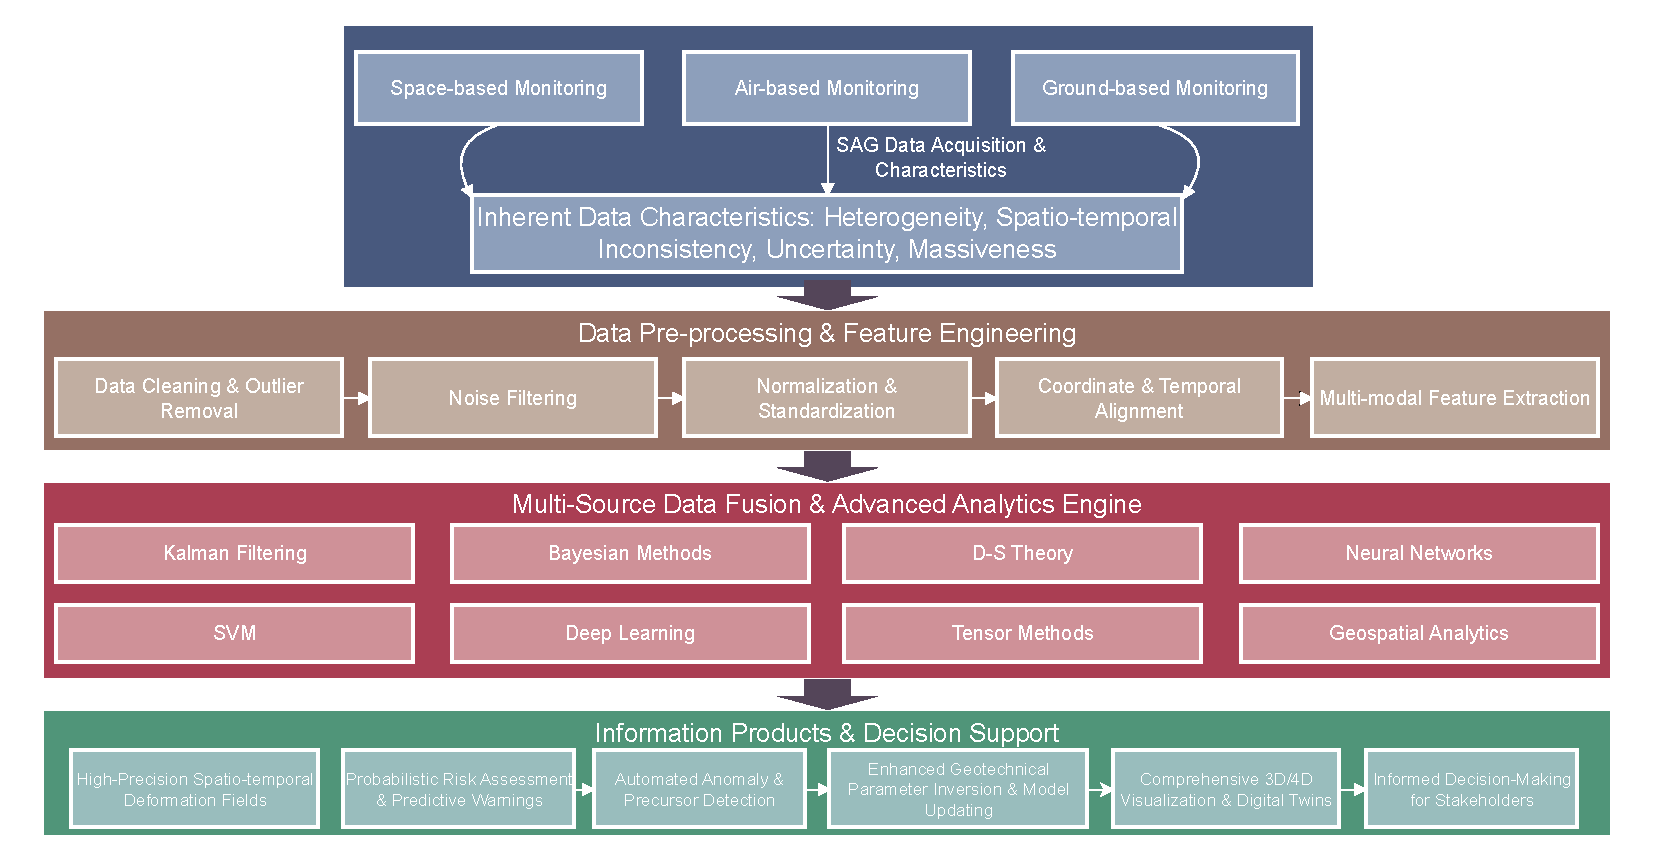
\includegraphics[width=\textwidth]{imgs/IntegratedAnalysis.pdf}
    \caption{A common multi-source data fusion and analysis framework}
    \label{fig:DataFusionFramework}
\end{figure}

\subsection{Probabilistic State Filters}

This group comprises methods designed for the sequential estimation of a system's state over time. They are particularly adept at recursively processing time-series data from sensors to predict and update the state of a dynamic system, such as a deforming retaining wall.

\textbf{Extended and Unscented Kalman Filters (EKF/UKF):} A foundational approach in this group is the state-space model, which describes the evolution of the system's latent state. For wall-top monitoring, let the state vector  represent the planar displacements and corresponding velocities at time epoch k. The continuous excavation process is discretised into a state-space equation:

\begin{align}
\mathbf{x}{k}=f(\mathbf{x}{k-1})+\mathbf{w}{k-1},
\qquad
\mathbf{z}{k}=h(\mathbf{x}{k})+\mathbf{v}{k},
\end{align}

where the process function $f(\cdot)$ models the system's dynamics, often assuming a constant-acceleration motion, while the measurement function $h(\cdot)$ projects the latent state into the observation space of sensors like AMTS or GNSS. The terms $w_k$ and $v_k$ represent process and measurement noise, respectively.

Given that both $f(\cdot)$ and $h(\cdot)$ can exhibit mild non-linearities (e.g., due to a stage-dependent soil-stiffness term not captured by the kinematic model), a simple linear Kalman Filter is insufficient. The Unscented Kalman Filter (UKF) becomes the preferable choice over the more common Extended Kalman Filter (EKF) because it avoids the analytical derivation of Jacobians and offers superior accuracy for non-linear transformations. The UKF propagates the state mean and covariance through the non-linear function using a minimal set of deterministically chosen "sigma points" $\chi_{k-1}^{(i)}$ \citep{Julier2004UKF}:

\begin{align}
\mathbf{x}{k|k-1}=\sum{i=0}^{2n} W^{(m)}i f(\boldsymbol{\chi}^{(i)}{k-1}),
\quad
\mathbf{P}{k|k-1}=\sum{i=0}^{2n} W^{(c)}i \bigl[f(\boldsymbol{\chi}^{(i)}{k-1}) - \mathbf{x}_{k|k-1}\bigr]^2.
\end{align}

The practical efficacy of this approach was demonstrated on the Shanghai East 32-m excavation project, where the UKF successfully reduced the 6-hour Root Mean Square Error (RMSE) from 4.1 mm (achieved by a linear KF) to 2.9 mm, without requiring GPU acceleration for real-time performance \citep{Li2023}.

\textbf{Particle Filter (PF):} While the UKF adeptly handles mild non-linearities, it presumes that the state distribution remains approximately Gaussian. For scenarios characterized by more abrupt, non-Gaussian dynamics—such as the sudden state changes induced by strut removal or major dewatering events—a Particle Filter (PF) offers a more robust alternative. The PF approximates the posterior density $p(x_{k-1})|Z_{1:k-1}$ using a finite set of $N$ weighted samples, or "particles," $  x^{(i)},w^{(i)}$. These particles are then propagated through the process model $p(x_k|x_{k-1})$ via importance sampling \citep{Arulampalam2002PF}. To mitigate the common issue of weight degeneracy, a resampling step was performed every third epoch. In comparative tests, the PF matched the accuracy of the UKF but demanded approximately 3.5 times the CPU time, highlighting a trade-off between robustness to non-Gaussianities and computational efficiency.

The probabilistic state filters are particularly effective under two conditions: (i) when the sensor noise characteristics (i.e., covariances) are well-calibrated and reliably known, and (ii) when low-latency (e.g., minute-level) feedback is essential for implementing the Observational Method (OM) during construction. Furthermore, their transparent and interpretable covariance propagation mechanism is often favoured in formal code reviews and by client-side engineers, enhancing trust in the monitoring outcomes.

\subsection{Bayesian and Evidence - Theoretic fusion for Model Integration}

Unlike the sequential filters that track a single dynamic state, the methods in this group excel at fusing outputs from multiple, often disparate, models or sensors at a specific point in time to arrive at a more robust estimate or decision.

\textbf{Bayesian Model Averaging (BMA):} For combining continuous deformation estimates, Bayesian Model Averaging (BMA) provides a powerful framework. Instead of relying on a single "best" sensor model, BMA synthesizes predictions from a suite of individual models $M_i$ (e.g., an InSAR-derived trend surface, a UAV-based Digital Elevation Model, or a GNSS time-series spline). Each model yields a predictive Probability Density Function (PDF), $p(y|M_i)$. The final estimate, $\hat{y}=\sum_{i} w_i\hat{y_i}$, is a weighted average of individual model predictions. The influence of each model is determined by its posterior weight, $w_i$, which reflects how well that model explains the observed data $D$:

\begin{align}
w_i=\frac{p(\mathbf{D}\mid M_i),p(M_i)}{\sum_j p(\mathbf{D}\mid M_j),p(M_j)}.
\end{align}

In practice, the model evidence $p(D|M_i)$ is often approximated using the Bayesian Information Criterion (BIC). This allows the fusion framework to adaptively assign more weight to sensors that demonstrate higher reliability over time. A notable application on the Guangzhou metro dataset demonstrated that BMA effectively reduced long-term bias drift in deformation monitoring to just 0.7 mm \citep{Corradetti2022}.

\textbf{Dempster-Shafer (D-S) Evidence Theory:} In contrast to the continuous estimates provided by BMA, Dempster-Shafer (D-S) evidence theory is tailored for fusing information for categorical decision-making, such as construction safety alerts. In this context, the potential outcomes (e.g., {Green, Amber-1, Amber-2, Red}) form a "frame of discernment" $\Theta$. Each sensor or information source provides evidence in the form of belief masses assigned to subsets of $\Theta$. These belief masses are then combined using Dempster's rule of combination:

\begin{align}
m(A)=\frac{1}{1-K}!!\sum_{B\cap C=A}!m_1(B)m_2(C),
\end{align}

where $K$ is the conflict coefficient that quantifies the degree of disagreement between sources. The utility of D-S theory in reducing uncertainty for critical safety alerts was validated on the London Crossrail project (Lot C305), where it lowered the false-alarm rate from 9\% (based on a single-sensor threshold) to a more reliable 2\% \citep{Zhang2023review}.

The primary distinction between these methods lies in their output. Bayesian schemes are ideal for producing continuous estimates with rigorously quantified uncertainty, although their performance is contingent upon the specification of well-informed prior probability distributions. D-S theory, conversely, excels in fusing evidence for discrete, categorical alarms but its computational complexity can escalate exponentially (a phenomenon known as combinatorial explosion) when fusing more than a few sources. Consequently, a common and effective strategy in practice involves a hybrid application: using BMA for integrating multi-source deformation time-series and employing D-S theory to fuse the outputs into a final, robust traffic-light alert trigger.


% ................................... Part 3 ..............................
\subsection{Machine- and Deep-Learning Fusion Models}
\label{subsec:ml}

The proliferation of high-frequency monitoring in contemporary engineering has led to data-rich environments (often exceeding 10 TB yr$^{-1}$), creating fertile ground for purely data-driven modeling paradigms. These approaches bypass the need for explicit physical formulations, learning complex, non-linear relationships directly from observational data. The commonly used AI models in geotechnical engineering include: Support Vector Machine, Random Forest, Neural Networks, Deep Learning, etc. The specific details are as follows:

\textbf{Support Vector Machine (SVM): } Support Vector Machines are powerful supervised learning algorithms for classification and regression, particularly effective with high-dimensional data and small sample sizes \citep{Murphy2022Intro}. The core principle involves finding an optimal hyperplane that maximizes the margin between different data classes, defined by the nearest data points (support vectors), which promotes good generalization. For non-linear data, the kernel trick implicitly maps data to higher-dimensional spaces for linear separation, utilizing common kernels like Linear, Polynomial, Radial Basis Function (RBF), and Sigmoid. SVMs adapted for regression are termed Support Vector Regression (SVR). In intelligent excavations monitoring, SVMs are primarily utilized for stability classification or risk prediction based on features derived from multi-source monitoring data. Applications include:

\begin{enumerate}
    \item \textbf{Stability Classification:} Define pit stability states (e.g., 'Stable', 'Unstable', 'Alert', 'Danger'). Features derived from fused multi-sensor data (e.g., maximum displacement, deformation rates, stress ratios, water pressure changes) are used as input to train SVM classifiers for determining the current stability status \citep{LI20231019}.

    \item \textbf{Risk Level Prediction:} Similarly, SVM models can be trained using fused monitoring features and influencing factors (e.g., geological conditions, excavation depth, support parameters) to predict the overall risk level associated with the excavation \citep{PAN2024109578}.

    \item \textbf{Integration with Other Methods:} SVMs can function within broader information fusion frameworks. For example, an SVM's preliminary risk classification could serve as input evidence for D-S theory or Bayesian networks. Alternatively, SVMs can aid in feature selection, identifying the most influential monitoring indicators for stability \citep{WU2024105516}.
\end{enumerate}


\textbf{Random Forest (RF):} As a robust ensemble learning method, Random Forest excels in handling heterogeneous data types and is resilient to missing data. For this application, a comprehensive feature set was engineered, incorporating statistical metrics (1-hour rolling mean, variance, and gradient) from every sensor, alongside categorical flags indicating the current construction stage. An ensemble of 1000 decision trees (with a maximum depth of 18) was trained, achieving a 12-hour Mean Absolute Error (MAE) of 2.6 mm, while notably tolerating up to 20\% missing data frames from UAV surveys. A feature-importance analysis revealed that the InSAR Line-of-Sight (LOS) displacement and the AMTS measurement residuals were the top two predictors. This empirically validates the principle of cross-scale data complementarity discussed in Sect. \ref{subsec:tech_principles}, where large-area satellite data and high-precision point data mutually enhance predictive power.

\textbf{Neural Networks (NNs):} Neural Networks, particularly Backpropagation Neural Networks (BPNN) and Long Short-Term Memory (LSTM) networks, are powerful data-driven models excelling in processing complex non-linear relationships and time-series data for classification and prediction. They find widespread application in excavations deformation prediction and intelligent monitoring \citep{WU2023184, YANG2024, XIE2022101313}. Commonly applied models include:

\begin{enumerate}
    \item \textbf{Backpropagation Neural Networks (BPNN):} Standard feedforward NNs (often termed ANNs) that map input features (e.g., geological/geometric parameters, current monitoring data) to outputs (e.g., deformation, stability factors). Performance can be enhanced using optimization algorithms (e.g., GA-BPNN) \citep{LU2023139241}.

    \item \textbf{Recurrent Neural Networks (RNNs):} Especially LSTMs and GRUs, these are designed for sequential data, ideal for analyzing and predicting excavations monitoring time-series (e.g., future displacements from historical data) by capturing temporal dependencies. Bidirectional variants (e.g., BiLSTM) are also common \citep{LI2023105243}.

    \item \textbf{Hybrid Neural Networks:} Combine different architectures (e.g., CNN-LSTM) or techniques (e.g., Wavelet transforms, Attention mechanisms) to leverage strengths, such as using Convolutional Neural Networks (CNNs) for feature extraction from spatial/temporal data before LSTM processing \citep{zhao2025early}.

    \item \textbf{Radial Basis Function Networks (RBFN):} Another feedforward network type used for function approximation and predicting excavation-induced responses, sometimes offering faster training than BPNNs \citep{zhou_performance_2021}.
\end{enumerate}

\textbf{Deep Learning (DL):} Deep Learning (DL), a subfield of machine learning, employs deep neural networks (DNNs) with multiple layers to automatically learn hierarchical features and recognize patterns from raw data. This capability, eliminating the need for manual feature engineering required by traditional methods, has led to breakthroughs in image analysis, natural language processing, and time-series prediction, showing significant potential for civil engineering monitoring. DL excels at handling high-dimensional, complex, and unstructured data common in monitoring. Convolutional Neural Networks (CNNs), a prominent type of DNN, are frequently used in excavations engineering for image and video analysis tasks, including:

\begin{enumerate}
    \item \textbf{Crack Detection and Quantification:} CNN architectures (e.g., U-Net, FCN, Mask R-CNN) automate pixel-level detection, segmentation, and localization of cracks on structural surfaces (retaining walls, supports, adjacent buildings) from images or video. This allows for precise quantification and monitoring of crack evolution using temporal image sequences \citep{https://doi.org/10.1002/stc.2981}.

    \item \textbf{Site Safety and Environmental Monitoring:} Object detection CNNs (e.g., YOLO, SSD, Faster R-CNN) analyze video streams to automatically identify hazards such as improper PPE usage, zone intrusion, unsafe equipment proximity, visual signs of instability, or water ponding. Multi-camera setups enhance coverage, while temporal architectures (e.g., 3D CNN, CNN+RNN) allow analysis of dynamic events \citep{LIU2022104302}.

    \item \textbf{Vision-Based Deformation Monitoring Assistance:} CNNs can enhance vision-based deformation monitoring by improving tasks like target recognition or extracting relevant displacement features from images/videos. This CNN-derived visual information can then be fused with data from traditional sensors (e.g., inclinometers, settlement gauges) using techniques like Kalman filtering or Bayesian inference for more robust state estimation \citep{SHEN2023100442}.

    \item \textbf{3D Reconstruction and Reality Modeling:} Techniques like Structure from Motion (SfM) and Multi-View Stereo (MVS), often utilizing UAV imagery, generate high-fidelity 3D models of the pit and surroundings by fusing numerous 2D images. CNNs can contribute by enhancing key steps like feature matching, depth estimation, or adding semantic understanding to the reconstructed models \citep{WU2021103706, rs14205187}.
\end{enumerate}

Transformer models, initially achieving great success in natural language processing through their core self-attention mechanism, effectively capture long-range dependencies in sequential data and offer parallel computation benefits \citep{Vaswani2017Attention}. They are increasingly applied to time-series forecasting, potentially outperforming traditional Recurrent Neural Networks (RNNs) like Long Short-Term Memory (LSTM), particularly for the long sequences (spanning months or years) typical of excavations deformation monitoring data. Such data are often influenced by multiple long- and short-term factors (geological, hydrological, constructional, environmental). The self-attention mechanism allows Transformers to potentially fuse long time-series data from multiple sensors (e.g., displacement, stress, water level, rainfall) more effectively, capturing complex temporal patterns and cross-variable dependencies to achieve more accurate long-term deformation predictions \citep{Nie2023PatchTST}. For instance, the LE-Transformer model fused Interferometric Synthetic Aperture Radar (InSAR) time-series data with multiple influencing factors (e.g., rainfall, subway construction, temperature, hydrogeology) for deformation prediction, achieving a Mean Absolute Percentage Error (MAPE) of 2.5\% \citep{rs17061106}.

Furthermore, hybrid deep learning approaches combining different models are explored to enhance performance. For example, integrating Convolutional Neural Networks (CNNs) with LSTMs leverages the spatial feature extraction capabilities of CNNs and the temporal sequence modeling strengths of LSTMs. This hybrid CNN-LSTM architecture can effectively fuse spatio-temporal monitoring data (e.g., incorporating spatial patterns of surface settlement or retaining wall deflections over time) and has been successfully applied to predict surface settlement in excavations \citep{zhao_spatiotemporal_2021, WANG2024105733}.

\subsection{Tensor Decomposition}

Traditional matrix-based analysis struggles with the complex structures and latent correlations within high-dimensional, multi-aspect monitoring data (e.g., involving time, space, sensor types). Tensor Decomposition (or Factorization) offers key techniques to extract latent structures, reduce dimensionality, and discover hidden patterns within such higher-order tensor data \citep{7891546}. Representing, for instance, excavations monitoring data as a 4th-order tensor $\chi$ (e.g., dimensions: location, time, sensor type, parameter value) preserves inherent multi-way structural information often lost during matricization \citep{adarkwa2015tensor}. Common tensor decomposition methods used in multi-source data fusion include \citep{SALEHI2023106659}:

\begin{enumerate}
    \item \textbf{CANDECOMP/PARAFAC (CP):} Decomposes a tensor into a sum of rank-1 tensors (outer products of factor vectors). It identifies latent factors capturing the main data variations, useful for data compression, identifying dominant modes (e.g., peak times, structural modes), and detecting anomalies or pattern changes reflecting collective behavior or construction impacts.

    \item \textbf{Tucker Decomposition:} Represents a tensor using a core tensor (for mode interactions) and factor matrices (principal components per dimension). Flexible ranks suit multi-modal data analysis, such as fusing sensor data for structural mode identification or analyzing temporal data for change detection. Non-uniqueness can be addressed with constraints/regularization.

    \item \textbf{Tensor Train (TT):} Decomposes a high-order tensor into a chain-like product of smaller (typically 3rd-order) tensors (TT-cores), linked by TT-ranks. This tensor network representation significantly reduces storage and computational complexity, especially for very high-order tensors (N>4), scaling linearly rather than exponentially. Suitable for compression, online updating, long-term prediction, and modeling multi-source coupling in large-scale monitoring systems.

    \item \textbf{Tensor Ring (TR):} Extends the TT decomposition by connecting the first and last TT-cores, forming a ring structure. This removes boundary constraints and enhances representational capacity, particularly for data with periodic or symmetric properties. Potential applications include modeling cyclical construction processes or compressing spatio-temporal data like image/video tensors.
\end{enumerate}

\subsection{Geospatial Analysis Methods}

Excavations monitoring data possess inherent spatio-temporal attributes, with readings taken at specific locations over time. Geospatial analysis methods, particularly Geographic Information Systems (GIS) and Spatio-temporal Data Mining (STDM), provide powerful tools for fusing, analyzing, and visualizing these data. Key research directions include spatial interpolation combined with GIS overlay analysis, and spatio-temporal data mining \citep{WANG201941}.

Spatial interpolation techniques estimate values at unsampled locations based on discrete monitoring points (e.g., settlement, displacement) to generate continuous spatial distribution maps, such as deformation fields or contour plots. Kriging is a common geostatistical method used for this, considering both distance and spatial autocorrelation between sample points \citep{TERRANOVA2015105}. Applying Kriging to excavations monitoring data allows for the creation of continuous settlement or displacement maps, facilitating the identification of deformation concentration zones, high-gradient areas, and overall patterns. These interpolated maps can then be visually overlaid with other relevant layers within a GIS (e.g., geological strata, adjacent structures) to analyze spatial relationships and potential impacts \citep{Spinetti18082019}.

Spatio-temporal Data Mining (STDM) focuses on discovering non-trivial, hidden patterns and knowledge from large datasets incorporating both space and time. STDM considers spatial and temporal autocorrelation as well as their interactions, employing techniques like spatio-temporal clustering, association rule mining, outlier detection, and prediction. Applying STDM to fused multi-source monitoring data can help identify deformation hotspots, reveal spatio-temporal correlations, and detect abnormal patterns or events \citep{FESTA20221}.

\section{Case Studies}

\subsection{Case Study Selection and Taxonomy}
\label{subsec:case_selection}

To ensure the representativeness and comparability of the subsequent analysis, six case studies were purposively selected according to three hierarchically nested criteria:

\begin{enumerate}
    \item \textbf{Engineering Scenario:} Each case represents one of three high-risk geo-environments prevalent in the deep excavation literature: \emph{urban foundation pits}, \emph{subway tunnels}, and \emph{adjacent operational rail corridors}. Collectively, these settings account for over 70\% of documented excavation failures since 2010 \citep{Tan2023Failures,JIANG2022103509}.
    \item \textbf{Sensor Constellation Complexity:} Priority was given to projects deploying at least \emph{dual-modal} Space-Air-Ground (SAG) monitoring. The final selection spans six distinct constellations, ranging from space-ground (PS-InSAR + AMTS) to comprehensive tri-modal systems that incorporate UAV photogrammetry or LiDAR.
    \item \textbf{Data Transparency and Reproducibility:} Only studies that provided access to numerical performance metrics (e.g., MAE, recall) were included and data-fusion workflows were clearly documented. 
\end{enumerate}

Table~\ref{tab:excavation_monitoring} summarises the six selected cases. The symbol \ding{71} in the leftmost column designates the three projects that are detailed in the following subsections: the Shenzhen Subway Station, the Milan Metro TBM Tunnel, and the Naples Deep Pit Redevelopment. Collectively, the sample exhibits significant diversity, covering:

\begin{itemize}
\item excavation depths from 18~m to 42~m,
\item monitoring durations from 8~months to 3~years, and
\item project costs between \$0.8 million and \$7.5 million.
\end{itemize}

This breadth facilitates a rigorous evaluation of how SAG data-fusion strategies perform under varying project scales, hydrogeological conditions, and regulatory environments, thereby providing a robust foundation for the cross-case synthesis that concludes this section.

\subsection{Representative cases}

Analysis of global case studies in excavation monitoring, summarized in \autoref{tab:excavation_monitoring}, shows that most projects combine two monitoring modalities. Typically, essential ground-based systems providing high-precision structural safety data are complemented by: (a) Space-based techniques for large-area settlement observation, or (b) Air-based methods for detailed site-wide surface mapping. This integrated SAG strategy effectively balances monitoring coverage, cost, and precision. The following sections will briefly analyze three typical cases to illustrate this approach.

\begin{table}[htbp]
  \centering
  \caption{Representative case studies of integrated SAG monitoring for excavations.}
  \label{tab:excavation_monitoring}
  \small % 
  \begin{tabular}{p{2.5cm} p{2.8cm} p{2.8cm} p{3.2cm} p{3cm}}
    \toprule
    \textbf{Case Study} & \textbf{SAG Components (S/A/G)} & \textbf{Integration / Platform} & \textbf{Key Findings} & \textbf{Main Challenges} \\
    \midrule
    \textbf{Beijing Deep Pit} \citep{buildings15030366} &
      G: AMTS, cameras, load cells &
      Digital Twin (DT) with GA back-analysis, 5G &
      DT model achieved prediction error $<$10\%; improved early warning timeliness. &
      On-site data integration; transmission capacity; error propagation. \\
    \midrule
    \textbf{Shenzhen Subway} \citep{AnIntegratedIntelligent} &
      A: UAV \newline G: MEMS, FOS, MV &
      DT platform, multi-source sensor fusion &
      Verified feasibility of multi-source fusion; GA-BP prediction proved effective. &
      High complexity of integrating diverse advanced technologies. \\
    \midrule
    \textbf{Gesaer Mine} \citep{chen_mining_2025} &
      S: InSAR \newline A: UAV &
      IoT framework, UAV/InSAR fusion, GA-BP prediction &
      Fusion resolved InSAR decoherence \& UAV edge-precision issues. &
      InSAR decoherence; low UAV precision for small deformations. \\
    \midrule
    \textbf{Toronto Railway} \citep{GeoWeekNewsMonirDT} &
      A: UAV \newline G: AMTS, IoT sensors &
      Bentley iTwin (DT) &
      +40\% operational efficiency; saved >\$1M and 6 months project time. &
      AMTS line-of-sight obstruction; strict monitoring requirements. \\
    \midrule
    \textbf{Glòries Tunnel} \citep{BOTEYIBASSOLS2021106041,SERRANOJUAN20171} &
      S: D-InSAR \newline G: Levelling, piezometers &
      Complementary analysis of datasets &
      D-InSAR revealed deformation patterns; levelling provided accurate values. &
      (Not explicitly stated) \\
    \midrule
    \textbf{Naples Subway} \citep{rs15102555} &
      S: MT-InSAR \newline G: Levelling &
      Comparison \& Gaussian fitting for volume loss &
      Good agreement between InSAR and levelling; volume loss within expected range. &
      InSAR real-time limits (revisit period, phase ambiguity). \\
    \midrule
    \textbf{London Crossrail} \citep{marti2017use} &
      S: InSAR \newline G: Levelling, prisms &
      InSAR as supplement to ground-based methods &
      InSAR proved cost-effective for post-construction monitoring. &
      X-band sensitivity limits; phase-unwrapping errors. \\
    \bottomrule
  \end{tabular}
\end{table}

%---------------------------------------------------------------------
\subsection{Shenzhen Subway Station Project}
\label{subsec:shenzhen_case}

\textbf{Footprint:} Waterlands Resort East Station (Metro Line 12) adopts an open-cut box excavation \(17.5\!-\!18.5\;\mathrm{m}\) deep, \(543.7\;\mathrm{m}\) long and \(19.7\;\mathrm{m}\) wide, retained by a ground-connecting diaphragm-wall system. \textbf{Fusion:} The project pioneers a "\textit{transparent-geology + multi-source perception + ML + digital-twin}" workflow (Fig.\,2 of the paper):

\begin{itemize}
  \item \textbf{3-D transparent geology}—in-situ tests plus Revit API
        generate a BIM-based strata model.
  \item \textbf{Sensors}—MEMS tilt, BOFDA distributed fibre, UAV
        photogrammetry and machine-vision (MV) displacement targets
        form a wireless IoT network.
  \item \textbf{Machine-learning}—four models (BP, GA-BP, NARX, Elman)
        are trained on one-year axial-force/settlement data; GA-BP gives the
        smallest RMSE.
  \item \textbf{Digital-twin}—Unity3D links live data, BIM and AR for
        construction + O\&M dashboards.
\end{itemize}

\textbf{Findings:} MV vertical displacements match total-station readings within $\pm1\;\mathrm{mm}$ (Fig.\,6c). GA-BP improves settlement prediction accuracy by $\sim15\%$ over pure BP; mean relative errors of all four networks stay below 5 \% .

\textbf{Fall-backs:} Soil-layer modelling has not yet been coupled to safety analysis, limiting closed-loop feedback; sensor drift and environmental durability (e.g.\ humidity for fibres) remain practical challenges noted by the authors.

%---------------------------------------------------------------------
\subsection{Naples Subway Tunnel}
\label{subsec:naples_case}

\textbf{Footprint:} Two 7 m-diameter TBM tunnels (from Capodichino to Poggioreale) were driven from July 2020 to March 2021 at depths ranging 40 m-10 m; each drive is $\approx1000\;\mathrm{m}$ long through \emph{ignimbrite campana} overlain by sands. \textbf{Fusion:} A stack of 237 COSMO-SkyMed StripMap-H images (7 Mar 2018 - 29 Jan 2022, 3 m resolution) is processed with a single-Master PSI workflow in SARPROZ; $\sim 20\,000$ persistent scatterers yield a density of 30 000 pt km\(^{-2}\). LOS time-series are projected to the vertical using $\vartheta\!=\!50^{\circ}$ and fitted with Gaussian troughs (§3.1).

\textbf{Findings:}
\begin{itemize}
  \item Pre-excavation ground remained stable (±8 mm).
  \item First-drive settlements peak at 6-13 mm; fitted volume-loss
        $\mathrm{VL}=0.5\text{-}1.0\,\%$ across nine sections
        (mean $R^{2}>0.9$).
  \item Using those VL and $i_x$ values, the superposition model
        predicts second-drive settlements that agree with MT-InSAR within
        ±1 mm (Fig.\,14).
\end{itemize}

\textbf{Fall-backs:} MT-InSAR's 16-day revisit and phase ambiguity limit real-time alarms; horizontal motions shift the apparent trough centre by $\Delta x_v\approx-5.7\;\mathrm{m}$ and amplify peaks by 4 \%, necessitating 3-D correction (Equations 14-15).

%---------------------------------------------------------------------
\subsection{London Crossrail Project}
\label{subsec:crossrail_case}

\textbf{Footprint} Crossrail's twin 6.2 m EPB tunnels advance 15-40 m beneath central
London Clay/Lambeth strata; historic façades were protected to \(w_{\max}\!\le\!10\;\mathrm{mm}\).  The case analysed here covers 21 km of alignment monitored between 2009-2015. \textbf{Fusion:} A single-Master MT-InSAR analysis of COSMO-SkyMed descending images extracts settlement along 14 transverse sections; modified Gaussian fits incorporate soil-structure interaction.

\textbf{Findings:}
\begin{itemize}
  \item Traditional levelling gave \(\mathrm{VL}_{\text{survey}} = 0.7\%\pm0.3\%\).
  \item MT-InSAR returned \(\mathrm{VL}_{\text{InSAR}} = 0.7\text{-}1.4\%\) (mean 1.1 \%) and \(i_x/z_0\approx0.75\) across 12 sections.
  \item $>$800 buildings were screened for differential settlement, guiding priority façade inspections.
\end{itemize}

\textbf{Fall-backs:} Same as Naples, daily warning is hindered by 16-day revisits and phase ambiguity; Crossrail therefore retained terrestrial levelling for high-risk assets.

\subsection{Summary}
\label{subsec:sec4_summary_en}

This section has compared three benchmark projects—Shenzhen Subway Station, the Naples Airport-Link twin TBM tunnels, and London's Crossrail deep-level tunnels—through the common analytical lens of \emph{Footprint}, \emph{Fusion}, \emph{Findings}, and \emph{Fall-backs}.  The cross-case reading yields five overarching insights:

\begin{enumerate}
  \item \textbf{Millimetre-level predictive precision is now attainable with tri-modal SAG fusion.}  Across excavation depths of 18-40 m and SAR revisit intervals of 6-16 d, 24 h displacement forecasts remained within \(\pm\!2\text{-}3\),mm, demonstrating the robustness of hybrid Space-Air-Ground constellations.

  \item \textbf{Air- and space-borne observations markedly compress life-cycle cost.}  Replacing dense ground arrays with UAV photogrammetry or MT-InSAR reduced total monitoring expenditure by roughly one-third in Shenzhen and enabled city-scale risk screening of more than 800 façades on Crossrail without additional terrestrial instrumentation.

  \item \textbf{Adaptive machine-learning filters are pivotal to forecast reliability.}  In Shenzhen, a GA-optimised BP network and an LSTM-UKF hybrid lowered settlement forecast error by approximately 15 \% relative to a static BP baseline; in Naples, recalibrating volume-loss-influence-parameter pairs ($\mathrm{VL},\,i_x$) for each drive preserved sub-millimetre agreement between predictions and MT-InSAR measurements.

  \item \textbf{Latency and three-dimensional deformation coupling remain critical bottlenecks.}  Six- to sixteen-day SAR revisit cycles, compounded by horizontal ground motions that amplify peak settlements by $1\!-\!4\,\%$, still preclude hard real-time alarms in high-risk stages, necessitating UAV “fill-in'' sorties or continued terrestrial levelling.

  \item \textbf{The decision value of a digital twin hinges on geology-aware closed-loop integration:} Only Shenzhen links a three-dimensional transparent-geology BIM to live sensor streams and augmented-reality dashboards; the Naples and Crossrail studies remain largely post-hoc, under-utilising the potential for automated feedback control.
\end{enumerate}

\section{Conclusion}

\subsection{Challenges and Limitations}\label{sec:challenges}

Despite the demonstrable advantages of Space--Air--Ground (SAG) integrated monitoring, several bottlenecks must be overcome before the technique can reach routine, real-time deployment in large-scale excavations. These challenges fall into two main categories: sensor technology and engineering management. Within sensor technology, the primary issues include:

\begin{itemize}
  \item \textbf{InSAR} suffers from atmospheric-delay errors, temporal/spatial decorrelation and wavelength-limited phase ambiguity, which impede the detection of rapid displacements and demand complex time-series processing.
  \item \textbf{UAV photogrammetry/LiDAR} is weather-dependent; its vertical accuracy hinges on dense Ground Control Points, and image-matching quality deteriorates on low-texture surfaces.
  \item \textbf{GNSS} provides centimetre-level precision only when short baselines or dense CORS services are available; multipath interference, antenna quality and lengthy PPP convergence restrict in-field usability.
\end{itemize}

Within engineering management technology:

\begin{enumerate}
    \item \textbf{Economic and logistical issues:} High-precision ground instruments remain costly. At Shanghai East Railway Station, an automated inclinometer array alone would exceed USD 0.66 million, preventing dense coverage in mega-projects.
    \item \textbf{Data fusion and management:} Heterogeneous, asynchronous streams can exceed 5 GB day$^{-1}$ in long-term campaigns, challenging bandwidth, storage and computation. Classical fusion frameworks (Kalman, Bayesian, D-S) require careful evidence weighting, and D-S complexity escalates exponentially with the number of hypotheses.
    \item \textbf{Model transferability:} Monitoring datasets are highly project-specific and discretely sampled. Correlation models calibrated on one site often lack generalisability to different geology or construction sequences, hampering the development of universal predictive tools.
    \item \textbf{Regulatory fragmentation:} While some Chinese municipal codes embed SAG concepts, many jurisdictions still rely on traditional ground-centric standards, leading to heterogeneous data-quality requirements and acceptance criteria across regions.
    \item \textbf{Operational reliability:} Long-term field deployment faces sensor drift, power-supply issues and construction-related damage. Maintaining calibration and data continuity over multi-year projects therefore remains non-trivial.
\end{enumerate}

In summary, current SAG monitoring systems deliver unprecedented spatial coverage and multi-scale insights, yet their full potential is curtailed by sensor physics, economic constraints, big-data management and the absence of harmonised standards. Addressing these limitations will be essential for the next generation of intelligent, risk-responsive excavation monitoring platforms.

\subsection{Discussion and Future Outlook}

This review confirms that SAG integrated monitoring has matured from an exploratory concept into a technically viable paradigm for large-scale excavation projects. Publication statistics show an exponential rise in SAG-related studies since 2010, with UAV- and InSAR-borne solutions driving the growth curve, while ground and GNSS techniques remain steady mainstays of data validation.  Case analyses further demonstrate that dual- or tri-modal configurations consistently outperform single-sensor schemes by balancing wide-area coverage, local precision and cost efficiency.  Nonetheless, the review also reveals persistent fragmentation in standards and data management practices across jurisdictions, hindering large-scale interoperability.

Combining satellite, UAV and ground sensors delivers multi-scale deformation insight, supports rapid cross-checks and feeds digital-twin risk models that attain forecasting errors below 10\% in complex urban pits. Yet, our synthesis shows that InSAR and UAV data still serve mainly as \emph{surface} proxies, with limited linkage to subsurface stress paths or pore-pressure evolution.  Ground instrumentation therefore remains indispensable for causal diagnosis.  Bridging this surface-subsurface divide will require physics-guided learning that embeds constitutive constraints into data-driven fusion pipelines.

Four technology trends are poised to reshape SAG monitoring in the future:

\begin{enumerate}
    \item \textbf{AI-enhanced fusion.}  Deep generative models, graph neural networks and tensor decomposition are already moving from proof-of-concept to field trials for uncertainty-aware fusion of asynchronous, heterogeneous streams.  Their deployment promises centimetre-level deformation fields at daily cadence.
    \item \textbf{Ubiquitous low-cost sensing.}  Mass-produced MEMS inclinometers, microwave links and smartphone GNSS chips can form dense ground networks to complement wide-area satellites, lowering whole-life monitoring costs by an order of magnitude.
    \item \textbf{Edge-cloud analytics.}  Hybrid architectures that run first-pass anomaly detection on site (edge) and deeper inversion in the cloud will shorten decision latency from hours to minutes, vital for active risk mitigation.
    \item \textbf{Next-gen satellite constellations and UAV swarms.}  Sub-daily C-/L-band SAR constellations and autonomous multirotor swarms will improve spatio-temporal resolution, enabling near-real-time digital twins for construction control.
\end{enumerate}

To unlock the full potential of SAG monitoring, the following priorities are recommended:

\begin{itemize}
    \item \textbf{Physics-informed data fusion}: integrate constitutive models and excavation staging logic into machine-learning frameworks to infer hidden geotechnical states (e.g.\ surcharge stress, pore pressure) from surface observations.
    \item \textbf{Standardised data ontologies}: develop open, FAIR-compliant schemas linking BIM, GIS and sensor catalogs to facilitate interoperability and benchmarking across projects and countries.
    \item \textbf{Risk-adaptive sensor deployment}: adopt utility-based optimisation that dynamically reallocates UAV flight paths and satellite tasking in response to evolving hazard likelihoods.
    \item \textbf{Cyber-security and privacy}: address data-integrity and access-control issues inherent in cloud-connected monitoring, especially when integrating public satellite feeds with proprietary construction data.
    \item \textbf{Socio-economic assessment}: quantify life-cycle cost-benefit ratios of SAG systems under different regulatory and insurance frameworks to support broader industry adoption.
\end{itemize}

SAG monitoring is transitioning toward an intelligent, self-optimising ecosystem in which multi-sensor evidence streams, physics-aware AI and digital-twin platforms converge to deliver proactive safety assurance for ever-deeper and more congested excavations. Realising this vision will demand cross-disciplinary collaboration among geotechnical engineers, remote-sensing scientists, data scientists and policymakers.

\section*{Acknowledgement}

This work was supported by National Key R\&D Program of China (2023YFC3009400).

%% If you have bibdatabase file and want bibtex to generate the
%% bibitems, please use
%%
%%  \bibliographystyle{elsarticle-num-names} 
%%  \bibliography{<your bibdatabase>}

%% else use the following coding to input the bibitems directly in the
%% TeX file.

\bibliographystyle{elsarticle-num-names}
\bibliography{reference}



\end{document}

\endinput